%\title{MS Thesis}
%\author{Emanuel Casiano-Diaz}
%\date{July 24, 2017.}

%\documentclass[12pt]{iopart}
%\pdfoutput=1
%\usepackage{iopams}

%\expandafter\let\csname equation*\endcsname\relax
%\expandafter\let\csname endequation*\endcsname\relax

%\bibliographystyle{iopart-num}
 %\usepackage[square,sort&compress]{natbib}
%Formatting Packages
\documentclass[12pt, two sided]{report}
\usepackage[utf8]{inputenc}
\usepackage[a4paper,top=1.1in,bottom=1.1in,left=1.6in,right=1.1in]{geometry}

%Math Packages
\usepackage{amsmath}
\usepackage{amssymb}
\usepackage{bm}
\DeclareMathOperator{\Tr}{Tr}

%Physics Package
\usepackage{physics}

%Allow accentuation marks
\usepackage[utf8]{inputenc}
\usepackage[T1]{fontenc}

%Image packages
\usepackage{graphicx}
\graphicspath{ {Images/} }

%Enumerating lists
\usepackage{enumerate}% http://ctan.org/pkg/enumerate

%Adjust depth of subsections
\setcounter{secnumdepth}{3}

%Adjust depth of table of contents
\setcounter{tocdepth}{3}

%References Packages
%\usepackage{biblatex}
%\addbibresource{references.bib}
\usepackage[bookmarks=true]{hyperref}
\hypersetup{
    hidelinks=true,
    linkcolor=blue,
    filecolor=magenta,      
    urlcolor=cyan,
}

%Commands and packages imported from particle entanglement paper
\usepackage{amsmath}
\usepackage{xcolor}
\usepackage{graphicx}
\usepackage{amssymb}

%\newcommand{\ket}[1]{\vert #1 \rangle}
\newcommand{\eket}[1]{\bigl \vert #1 \bigr \rangle}
\newcommand{\R}{\boldsymbol{R}}
\newcommand{\Rt}{\tilde{\R}}
%\newcommand{\bra}[1]{\langle #1 \vert}
\newcommand{\ebra}[1]{\bigl \langle #1 \bigr \vert}
\newcommand{\eexp}[1]{\bigl \langle #1 \bigr \rangle}
\newcommand{\figref}[1]{Fig.~\ref{#1}}
\renewcommand{\vec}[1]{\boldsymbol{#1}}
\newcommand{\ren}{R\'{e}nyi~}
\newcommand{\rnote}[1]{{\it \textcolor{red}{#1} }}
\newcommand{\Eqref}[1]{Eq.~\eqref{#1}}

%Copied from paper
\usepackage{color}
\usepackage{graphicx}
\usepackage[color=green!60]{todonotes}
\usepackage{physics}
\usepackage{amsthm}
\usepackage{amsmath}
\usepackage{amssymb}
\usepackage{enumerate}
\usepackage{placeins}
\usepackage{booktabs}
\usepackage{dsfont}

%For reference formatting
\usepackage[numbers,sort&compress]{natbib}
\bibliographystyle{nsf_new_url}

\setlength{\footskip}{22pt}
 
 %Line spacing
\usepackage{setspace}
\doublespace

\begin{document}
\sloppy

%%%%%%%%%%%%%%%%%%%% TITLE PAGE %%%%%%%%%%%%%%%%%%%%%%%%%%
\begin{titlepage}
	\begin{center}
		\vspace*{1cm}
		
		\begin{singlespace}	
		\Large
		%\textbf{Quantum Entanglement of One-Dimensional Spinless Fermions}
		QUANTUM ENTANGLEMENT OF ONE-DIMENSIONAL SPINLESS FERMIONS
		\end{singlespace}
		
		\vspace{0.9cm}
		
		%\vfill
		
		\normalsize
		A Thesis Presented \\
		\vspace{0.4cm}
		by \\
		\vspace{0.4cm}
		Emanuel Casiano-Diaz \\
		\vspace{0.4cm}
		to \\
		\vspace{0.4cm}
		The Faculty of the Graduate College \\
		\vspace{0.4cm}
		of \\
		\vspace{0.4cm}
		The University of Vermont
		
		\vspace{0.7cm}

		%\vfill
		
		\begin{singlespace}
		In Partial Fullfillment of the Requirements \\
		for the Degree of Master of Science \\
		Specializing in Physics	
		\end{singlespace}
		
		\vspace{0.5cm}
		
		May, 2019
		
	\end{center}
	
	\vspace{0.1cm}
	
	\begin{singlespace}
	\begin{flushright}
		Defense Date: March 28th, 2019. \\
		Thesis Examination Commitee:
		
		\vspace{0.15cm}
		
		Adrian Del Maestro, Ph.D, Advisor \\
		Christopher Danforth, Ph.D, Chairperson \\
		Dennis Clougherty, Ph.D \\
		Cynthia J. Forehand, Ph.D, Dean of the Graduate College
		
	
	\end{flushright}
	\end{singlespace}

\end{titlepage}

%%%%%%%%%%%%%%%%%%%%%%%%%%%%%%%%%%%%%%%%%%%%%%%%%%%%


%%%%%%%%%%%%%%%%%%%% TITLE PAGE %%%%%%%%%%%%%%%%%%%%%%%%%%

\pagenumbering{gobble}
\chapter*{Abstract}
The constituents of a quantum many-body system can be inextricably linked, a phenomenon known as quantum entanglement. Entanglement can be used as a resource for quantum computing, quantum communication and detecting phase transitions, among others. The amount of entanglement can be quantified via the von Neumann and R\'enyi entropies, which have their origins in information theory.
\\
\\
In this work, the quantum entanglement between two subsystems of a one dimensional lattice model of fermions is quantified. The von Neumann and R\'enyi entropies were calculated for two types of subsystems. In the first study, the subsystems were treated as two subsets of particles, and in the second, as two spatial subregions. Finally, by considering particle conservation rules, the amount of entanglement that can actually be accessed as a resource was calculated. In all cases, the quantum entanglement served to detect phase transitions in the model.  

\chapter*{Acknowledgments}
To my educators, for teaching me what I know today. To my incredible family for their never ending support. To my advisor, Adrian Del Maestro, for guiding my path as a graduate student and making the journey so enjoyable. And to Hatem Barghathi, for the countless hours spent teaching me about most of the topics that will be presented in this thesis and many more outside its scope.
\\
Thanks.
\\
\\
This research was supported in part by the National Science Foundation under Award No. DMR-1553991. Computations were performed on the Vermont Advanced Computing Core supported in part by NSF award No. OAC-1827314.

\pagenumbering{roman} % Roman numerals
\setcounter{page}{2}

\singlespacing
\tableofcontents
\doublespacing

\chapter{Introduction}
\pagenumbering{arabic}

\section{The $t-V$ Model}
\label{sec:t-VIntro}

So called "toy models" are ubiquitous in condensed matter physics. These describe a complex system in simple terms so that attention can be given to an underlying mechanism of such system. The Ising model, in it simplest form, can describe how a system spontaneously becomes a ferromagnet by considering interactions between quantum spins and tuning an external temperature. Similarly, the Hubbard model considers the interaction strength of electrons on a lattice and a hopping rate to describe the transition between conductor and insulator. The fact that the two aforementioned examples mention phase transitions is not mere coincidence. 

Near a phase transition, small set of parameters governs macroscopical physical behavior, a phenomenon known as universality. Different systems having the same value for such universality parameters are said to fall under the same universality class. 

The studies that will be presented in this thesis are concerned with a specific model, which shall be referred to as the $t-V$ model. This model, is equivalent to the $XXZ$ spin model and describes $N$ itinerant spinless fermions on a 1D lattice of size $L$. These fermions can tunnel to neighboring sites and the rate at which they do so is proportional to a hopping parameter $t$. An interaction potential, $V$, between the fermions is also considered, which could be repulsive ($V > 0$) or attractive ($V < 0$). Periodic and anti-periodic boundary conditions will be assumed for the case of odd and even particles, respectively. Mathematically, this is represented by the following Hamiltonian:
%
\begin{equation}
H = -t \sum_{i} \left ( c_{i}^{\dag} c_{i+1}^{\phantom{\dag}} + c_{i+1}^{\dag} c_{i}^{\phantom{\dag}} \right )+ V \sum_{i} n_i n_{i+1}   
\label{eq:t-VHamiltonian}
\end{equation}
%
where $c_{i}^{\dag}$ ($c_{i}$) creates (annihilates) a fermion on site $i$ and $n_{i} = c_i^{\dag}c_i^{\phantom{\dag}}$ counts the number of fermions on site $i$. Formally, these creation and annihilation operators are defined such that the following anticommutation relations are satisfied:
%
\begin{equation}
\label{eq:commutationRelations}
\left \{ c_i^{\dag} , c_j^{\dag} \right \} = 0 \text{  }, \text{  }
\left \{ c_i , c_j\right \} = 0 \text {  } , \text{  }
\left \{ c_i^{\phantom{\dag}} , c_j^{\dag} \right \}  = \delta_{ij},
\end{equation}
%
where $\delta_{ij}$ is the Kronecker-Delta function. For example, in the case that there's no fermion on the site in which the creation operator acts, then $c^{\dag} \ket{0} = \ket{1}$. The interaction term can then be understood conceptually as adding to the potential energy of the system if there are multiple particles in neighboring sites. Conceptually, the first term may be more difficult to understand in its current representation, due to this operator being non-diagonal. Nevertheless, expressing it in the momentum basis, where it is diagonal, illustrates that how contributions to the kinetic energy come from all particles with nonzero momentum (which will be all of them unless $t=0$). A detailed mapping of the kinetic energy operator from lattice site to momentum basis can be seen in Appendix \ref{appendix:kineticMapping}.

%%%%%%%%%%%%%%%%%%%
\begin{figure*}[h]
\begin{center}
\includegraphics[width=1.0\textwidth]{phaseDiagramtV.pdf}
\end{center}
\caption{Phase diagram of the $t-V$ model accompanied by pictures of candidate ground states for $N=2$ fermions on a $L=4$ site lattice. For the purposes of measuring accessible entanglement, the lattice has been bipartitioned into spatial subregions $A$ (blue) and $B$ (red), each of size $\ell = 2$. We assume periodic boundary conditions. In the limit of strong attractive interactions where $V/t \ll -2$, the particles cluster together and there are $L$ equally probable configurations corresponding to all translations of the cluster.  At the first order phase transition where $V/t = -2$, all ${L}\choose{N}$ configurations are equally probable resulting in a flat state. In the TLL phase with $|V/t| < 2$,  particles are delocalized and we have included a characteristic state corresponding to free fermions $(V=0)$. In the limit of strong repulsive interactions where $V/t \gg 2$, fermions maximize their distance from each other resulting in a charge density wave (CDW) phase. The open and closed circles on the $V/t$ axis denote a first order and continuous phase transition, respectively.}
\label{fig:phaseDiagram}
\end{figure*}
%%%%%%%%%%%%%%%%%

Figure \ref{fig:phaseDiagram} shows the phase diagram of the $t-V$ model. For $V/t \ll -2$, the fermions cluster together due to the strong attractive interaction. The state in this regime is an equal superposition of all possible such cluster configurations over all lattice sites. At $V/t = -2$, the system undergoes a first order phase transition into the Tomonaga-Luttinger Liquid (TLL) phase. Here, the state is in a superposition of all possible configurations of the fermions on the lattice, with the weights of each being different, in general. At $V/t = 2$, the system undergoes a continuous phase transition into the charged density wave (CDW) phase. At $V/t \gg 2$, the strong repulsion between particles leads to them forming an alternating pattern of particle-vacancy-particle- \dots The state in this regime becomes an equal superposition of the only two possible such configurations.

Notice that in Figure \ref{fig:phaseDiagram} the lattice sites have two different colors, blue and red. This is to illustrate that a system can be partitioned into smaller subregions. In this particular example, each partition would be of size 2 lattice sites. In fact, subdividing a system into this smaller subsystems will be necessary for the main phenomenon of interest in this thesis: quantum entanglement. The bulk of this work will consist of quantifying the amount of entanglement of a system via entropy measures. Before getting to explaining entanglement, in the next section, an overview of entropy or information measures will be given.

\section{Information measures}
\label{sec:informationMeasures}

	The probabilistic nature of quantum mechanics, provides an ideal test bed for entropy measures. In section \ref{sec:t-VIntro}, it was mentioned that knowing something about $A$, will give you information about its entangled pair $B$. The amount of information gained in such measurement can be quantified by the entropy of a subsystem. Recall that, in essence, entropy is related to the disorder of a system. Thus, doing a measurement on a high entropy state, will give more information than in a highly ordered state, in which the outcome of the measurement is more like to be known a priori. For this reason, entropy measures will be referred to as information measures for the remainder of this work.
	
	In the next section, the information measure used to quantify entanglement, will be introduced. Then, the actual measures of entanglement will be presented.
	
	\subsection{Shannon entropy}
	
	The Shannon or information entropy is the average amount of information gained from a a data set in which the entries occur according to some probability distribution. It is defined as:
	%
	\begin{equation}
	S = -\sum_{i} p_i \log_{b} p_i
	\label{eq:shannonEntropy}
	\end{equation}
	%
	where the sum is carried over all entries in the data set and $p_i$ is the probability of measuring entry $i$. The base $b$ can be chosen arbitrarily depending on the context. The base will be chosen as the number $e$ such that $\log_b \to \ln$ for the remainder of this work. Up next, a hopefully simple example will be presented in order to give some intuition about how information gain can be estimated with Eq.~(\ref{eq:shannonEntropy})
	
	Consider a regular coin flip. Disregarding all physical effects that can somehow bias the outcome, it is expected that either heads or tails will randomly occur with equal probability $1/2$. Then, since there is no bias towards any of the two possible outcomes of the coin flip, the information gain should be at a maximum. The Shannon entropy for this case is:
	%
	\begin{align}
	S &= -\frac{1}{2} \ln{\frac{1}{2}} - \frac{1}{2} \ln{\frac{1}{2}}  \nonumber\\
	&= \ln{2}  \nonumber \\
	S &\approx 0.6931 \nonumber \dots
	\end{align}
	%
	In base 2, this would correspond to a whole bit of information gained in the coin measurement. Now, consider a coin that has been modified in such a way that it is more likely to get one outcome than the other. For the sake of this example, let's say that heads shall occur with probability $2/3$, while tails with $1/3$. Then, since it is two times more likely that heads will occur instead of tails, more certainty about the outcome is known beforehand and thus the information gained decreases. Shannon entropy gives:
	%
	\begin{align}
	S &= -\frac{2}{3} \ln{\frac{2}{3}} - \frac{1}{3} \ln{\frac{1}{3}} \nonumber \\
	S &\approx 0.6365 \dots \nonumber
	\end{align}
	%
	Finally, an extreme case would be a coin that was incorrectly manufactured and has heads on two sides. Opposite to a regular coin, in which maximum information is gained because both heads and tails have the same probability, the probability for heads to land in this case is 1, while 0 for tails. Since the result is already known before the coin flip, the information gain after the coin flip is none. Shannon entropy gives:
	%
	\begin{align}
	S &= -1\ln{1} = 0 \nonumber
	\end{align}
	%	

	Now that some intuitive examples were discussed, the quantum information theory counterpart of Shannon's entropy will be presented.
	
	\subsection{von Neumann entropy}
	
	In calculating the Shannon entropy, the probabilities of random events occurring are required. The probabilities of finding a system in a certain state can be encoded in its density matrix. The density matrix is defined as:	
	%
	\begin{align}
	\label{eq:densityMatrix}
	\rho = \vert \Psi \rangle \langle \Psi \vert
	\end{align}
	%
	where $\vert\Psi\rangle$ is the state of the full system, such that $\vert \Psi \rangle \in \mathcal{H} = A \otimes B$ and the normalization condition on the states of the system imply that $\Tr \rho = 1$. The state $\vert \Psi \rangle$ can be partitioned into subregions or subsystems that live in Hilbert Space $A$ and $B$, respectively. The von Neumann entropy measures the information gained about subsystem $B$ by doing a measurement on subsystem $A$. The von Neumann entropy is defined as:
	%
	\begin{equation}
	S = -\Tr\rho_{A} \ln{\rho_A}
	\label{eq:vonNeumannEntropy}
	\end{equation}
	%
	where $\rho_A$ is known as the reduced density matrix of subsystem $A$ and it is obtained by tracing out the degrees of freedom in $B$, an operation known as the partial trace (with respect to $B$, in this case). The reduced matrix of $A$ is then:
	%
	\begin{equation}
	\rho_{A} = \Tr_B \rho = \sum_b \langle \psi_b \vert \Psi \vert \psi_b \rangle
	\label{eq:partialTrace}
	\end{equation}
	%
	where the sum is carried over all possible states in which subsystem $B$ can be in and $\psi_b$ denotes each of these states. Normalization implies that $\Tr \rho_A = 1$.
	
	The von Neumann requires access to the density matrix of the system. The density matrix can be obtained via exact diagonalization of the ground state Hamiltonian (see Appendix \ref{app:lanczos} for details on Lanczos diagonalization). For large systems though, exact diagonalization is not feasible due to the exorbitant amount of memory required and quantum Monte Carlo (QMC) methods must be employed. In QMC methods, there is no access to the reduced density matrix, but the expectation value of a unitary operator that swaps the $A$ states between two identical copies of a system gives higher powers of the reduced density matrix \cite{Hastings:2010dc}. In other words, $\rho_{A}$ is not accessible but $\rho_{A}^{\alpha}$ can be obtained for $\alpha > 1$. It was also shown experimentally \cite{Islam:2015cm}  that $\rho_A^{\alpha}$ can be obtained by interference of two identical copies of ultra-cold atoms. Thus, a new formulation of the entropy must be introduced that depends on higher powers of $\rho$.
	
	\subsection{R\'enyi entanglement entropy}
	
	In order to calculate entropy via QMC or experimentally \cite{Hastings:2010dc, Islam:2015cm}, a measure that depends on powers of the reduced density matrix larger than 1 must be used, since these methods do not have access to the reduced density matrix. The R\'enyi entanglement entropy, which is the analogue of the R\'enyi entropy from information theory, provides an information measure that depends on $\rho_{A}^{\alpha}$ instead of $\rho_{A}$. The R\'enyi entanglement entropy is defined as:
	%	
	\begin{equation}
	\label{eq: renyiEE}
	S_{\alpha} = \frac{1}{1-\alpha} \ln \Tr \rho_{A}^{\alpha}
	\end{equation}
	%
	where $\alpha$ is known as the R\'enyi index. In the limit of $\alpha \to 1$, the R\'enyi entanglement entropy becomes to the von Neumann entropy. Higher R\'enyi indices will result in lower R\'enyi entanglement entropies, as shall be discussed up next.
	
	Due to the normalization conditioned imposed on the reduced density matrix, the sum of its eigenvalues must also be unity. Each of the eigenvalues must then belong to the closed interval $\left [ 0,1 \right ]$. Raising $\rho_A$ to a power $\alpha > 1$ is equivalent to raising each eigenvalue by $\alpha$ and as a result, the trace of $\rho_A$ will decrease. A lower trace of $\rho_A$ will then make the R\'enyi entanglement entropy lower. Thus, $S_{\alpha}$ is a monotonically decreasing function of $\alpha$. 
	
	Now that the $t-V$ model and the information measures have been introduced, it is time to discuss quantum entanglement itself.
	
\section{Quantum entanglement}
\label{sec:quantumEntanglement}

	A quantum many body system is entangled if its constituents present correlations that cannot be classically described. 	Mathematically, a quantum many-body system is entangled if it cannot be factored into a tensor product of the state of subsystems $A$ and $B$. The condition for entanglement is then,
%	
	\begin{equation}
	\vert\Psi\rangle \neq \vert\Psi_{A}\rangle \otimes \vert\Psi_{B}\rangle
	\label{eq:entanglementCondition}
	\end{equation}
%
	Assuming subsystems $A$ and $B$ are entangled with one another, knowing something about $A$ automatically gives you some knowledge of $B$. Since the average information gained about $B$ when measuring $A$ can be quantified via von Neumann and R\'enyi entanglement entropies, these can be used as indication of how entangled the two subsystems are with each other. A system is highly entangled if its state possesses a large entanglement entropy.
	
	%%%%%%%%%%%%%%%%%%%
\begin{figure*}[h]
\begin{center}
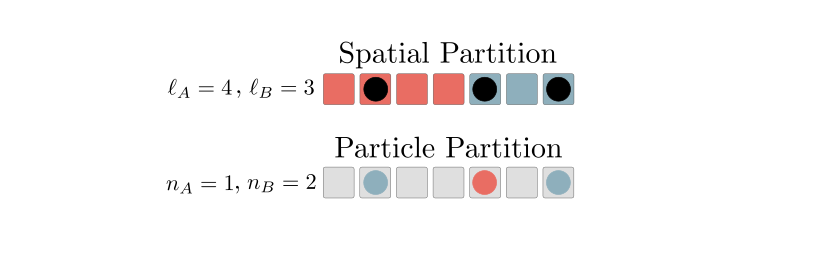
\includegraphics[width=1.0\textwidth]{spatialParticle.pdf}
\end{center}
\caption{Schematic of a one-dimensional lattice of $L=8$ sites and $N=4$ particles under two types of bipartitions. The top lattice is bipartitioned into two spatial subregions $A$ (red) and $B$ (blue). The size of both subregions is $\ell_A = \ell_B = 4$ sites. The bottom lattice is bipartitioned into two subsets of identical particles. Subset $A$ consists of only $n_A=1$ particles, while $B$ consists of $n_B = N - n_A = 3$.}
\label{fig:spatialParticle}
\end{figure*}
	%%%%%%%%%%%%%%%%%%%

	
	The subsystems in which a system is partitioned can represent subsets of particles or quantum modes. The modes can represent spatial subregions, momenta, spins, etc... Since the case of entanglement in the $t-V$ model under a spatial bipartition was studied in this work, from here onwards, the mode partition shall be referred to as a spatial partition. Up next, an overview of particle-partitioned and spatially-partitioned entanglement is given.

	
	A many-body system can be partitioned into subsets of particles. In the case of a particle bipartition, one of the subsets will have $n$ particles and its complementary subset, $N-n$ particles, where $N$ is the total number of particles in the system. To quantify entanglement between the subsets of particles, the $n-$body reduced density matrix ($n-RDM$) is used:
	%
	\begin{equation}
	\rho_{n} = \int dx_{n+1} \dots \int dx_N \langle x_{n+1} \dots x_N \vert\Psi\rangle \langle\Psi\vert x_{n+1} \dots x_N \rangle
	\label{eq:nBodyDensityMatrix}
	\end{equation}
	%
	where $\vert\Psi\rangle$ is the first quantized wavefunction of a system of $N$ identical particles and it properly anti-symmetrized or symmetrized for fermions and bosons, respectively.  The entanglement of a system under a particle bipartition allows to measure non-local effects, complementing the study of spatial entanglement. 
	In measuring spatial entanglement, a system is bipartitioned into a spatial subregion of size $\ell_{A}$ and a complementary region size $L - \ell_A \equiv \ell_B$. Under this type of partition, states are represented in second quantization. In other words, a state $\vert\Psi\rangle = \vert n_1 \rangle \otimes \vert n_2 \rangle \dots \otimes \vert n_N \rangle$ is characterized by the set of occupation numbers on each site. In the case of fermions, 0 and 1 correspond to a vacant and occupied site, respectively.  Figure \ref{fig:spatialParticle} illustrates schematically a $1D$ lattice of size $L = 8$ and $N = 4$ under a spatial and then a particle bipartition.
	
	\subsection{Accessible Entanglement}
	Whether it's under a particle or spatial bipartition, the goal is to use the entanglement present in a system as a resource. The von Neumann and R\'enyi entropies provide mathematical quantification of the entanglement of a system. Nevertheless, for physical applications, superselection rules (SSR), such as particle number and spin conservation must be considered.  An SSR, restricts the possible quantum states that can be obtained after measurement. For illustration of an SSR, take the example of $N$ particles on a $1D$ lattice partitioned into two spatial subregions $A$ and $B$. If initially there are $n$ particles in the sites belonging to subregion $A$ then, after measurement, the positions of the particles could change, but the number of particles in $A$ will still be $n$. In this case, a local particle number SSR has been imposed. In Ref.~\cite{Wiseman:2003jx}, a new formulation for the entanglement was proposed that takes this particle number SSR into account.
	
	For a quantum many-body system subject to physical laws conserving some quantity (particle number, charge, spin, etc.), the set of local operations on the state $\ket{\Psi}$ are limited to those that don't violate the corresponding global superselection rule.  For simplicity, attention will be focused to the case of fixed total particles $N$ and thus we are restricted to only those operators which locally preserve the particle number in $A$.  The effect this has on the amount of entanglement that can be transferred to a qubit register is apparent from the simple example (adapted from Ref.~\cite{Wiseman:2003jx} of one particle confined to two spatial modes $A$ and $B$ corresponding to site occupations.  Then, for the state $\ket{\Psi} = \left(\ket{1}_A \otimes \ket{0}_{B} + \ket{0}_A \otimes \ket{1}_{B} \right)/\sqrt{2}$, Eq.~\eqref{eq:vonNeumannEntropy} gives that $S_1 = \ln 2$. However, this entanglement cannot be transferred to a register prepared in initial state $\ket{0}_R$ via a $\texttt{SWAP}$ gate:
\begin{align*}
    & \texttt{SWAP} \ket{0}_R\otimes\left(\ket{1}_A \otimes
    \ket{0}_{B} + \ket{0}_A \otimes \ket{1}_{B} \right)/\sqrt{2} \\
    &= \frac{1}{\sqrt{2}} ( \ket{1}_R \otimes \underbrace{\ket{0}_A \otimes \ket{0}_{B}}_{N\neq1} + \ket{0}_R \otimes \underbrace{\ket{0}_A \otimes \ket{1}_{B}}_{N=1})
    % &= \frac{1}{\sqrt{2}}\ket{0}_R \otimes \ket{0}_A \otimes
    %     \ket{1}_{B}
\end{align*}
The $\texttt{SWAP}$ gate in the example above takes the register modes and exchanges them with the modes in subsystem $A$ of the resource:
%
\begin{equation}
\texttt{SWAP} \ket{\phi}_R \otimes \ket{\psi}_A = \ket{\psi}_R \otimes \ket{\phi}_A
\end{equation}
%
The $\texttt{SWAP}$ can be defined such that it exchanges resource modes with modes in $B$ instead. Notice that the first term post $\texttt{SWAP}$ in the example preserves particle number in the resource, since there is a total of 1 particle in $A$ and $B$. But, the last term is not physically allowed since it has no particles at all in $A$ and $B$, thus violating the restriction that total particle number be fixed. The state of the register post-swap will remain in a product state, meaning that the amount of entanglement that can be accessed as a resource is identically zero. In general, it will be seen that the amount of accessible entanglement will be less or equal than the full entanglement of the system.

Formally, the accessible entanglement is defined as:
%
\begin{equation}
\label{eq:accS1}
S_1^{\rm acc} = \sum_n P_n S_1(\rho_{A_{n}})
\end{equation}
%
where the sum is carried over all possible local particle numbers of $A$, $P_n$ is the probability that subsystem $A$ will have $n$ particles, $S_1$ is the von Neumann entropy, which will be a function of $\rho_{A_{n}}$. Notice the additional subscript $n$ in the reduced density matrix expression. Whereas for the full entanglement entropy, knowing $\rho_A$ would suffice, for the accessible entanglement entropy, the reduced density matrix must be also be projected onto the subspace of local particle number $n$. Additionally, recall that the normalization condition asks for $\sum_n P_n = 1$. This accessible entropy was originally only well defined for the von Neumann entropy $S_1$. Recently, a generalized version of the accessible entanglement that works for R\'enyi indices greater than 1 was proposed \cite{Barghathi:2018oe}, such that any accessible R\'enyi entropy can now be calculated.

Now that all the ground work for the results presented in this thesis has been introduced, an outline of the remaining chapters is given. In chapter 2, the particle-partitioned entanglement entropies in the $t-V$ model will be studied. By neglecting the exact entanglement entropies of free fermions, the contribution to particle entanglement coming from particle interactions is calculated. It is also seen that results from exact diagonalization agree with predictions coming from Tomonaga-Luttinger Liquid (TLL) theory. Chapter 3 will present computational results that support the generalization of the accessible R\'enyi entropies, this time under spatial bipartitions of the $t-V$ model. A power-law scaling is suggested for a peak near the continuous phase transition of the model. Then, the difference between full and accessible entanglement entropies is computed at various regimes of the model and it is shown that the probability of finding a number of particles $n$ in one subregion of the system after measurement follows a Gaussian distribution in the TLL regime. Finally, chapter 4 will briefly discuss some unanswered questions that have emerged from the projects presented here and future ones will be discussed and a thesis summary is provided.




	

	


\chapter{Particle Partition Entanglement in the $t-V$ Model}
\section{The operational entanglement}

Consider some $N$-particle quantum state, in which the $N$ particles are shared between spatial subregions $A$ and $B$, or Alice and Bob, if you will. If Alice's and Bob's particles are entangled, this entanglement could be used as a resource for real world applications. Nevertheless, by using the traditional Von Neumann or R\'enyi Entanglement entanglement entropy, an overestimated measure of the physically available entanglement is obtained. This happens because for applications that rely on quantum entanglement, the particle number has to be conserved and these traditional measures do not account for this. To address this issue, Wiseman and Vaccaro \cite{PhysRevLett.91.097902} developed a measure known as Operational Entanglement (originally called Entanglement of Modes by the authors). The operational entanglement takes into account that the local particle number that are in Alice and Bob has to be conserved, giving a more physically accurate measure of entanglement.

	\subsection{Projecting onto subspaces of fixed local particle number}
	
	Knowing the density matrix of subregion $A$ will suffice to calculate, for example, the spatial R\'enyi Entanglement Entropy. Nevertheless, to get the operational entanglement, simply knowing $\rho_{A}$ is not enough. To recap, the spatial R\'enyi Entanglement Entropy is given by:
	

\begin{equation}
 S_{\alpha}(\rho_{A}) = \frac{1}{1-\alpha} \log{\Tr{\rho_{A}^{\alpha}}} 
\end{equation}

Where $\alpha$ is the R\'enyi Index and $\rho_{A}$ is the density matrix of subregion $A$. This calculation is still required to get operational entanglement but, as shall be seen, a few extra steps have to be taken to make sure that local particle number conservation is being satisfied. The first of these extra steps will be to project $\rho_{A}$ to subspaces of local particle number. Projection operators can be written as diagonal matrices with ones on the columns corresponding to the subspace for which the projection is desired. Knowing this, the projection operators into subspaces of fixed local particle numbers can be built rather simply. The projected reduced density matrix of  $A$ into the subspace of fixed local particle number $n$ is obtained by:

\begin{equation}
\rho_{A,n} = \frac{1}{P_n} \hat{\Pi}_n \rho_A \hat{\Pi}_n
\end{equation}

Where $P_n$ is the probability of measuring an Alice state with $n$ particles and $\hat{\Pi}_{n}$ is the projection operator onto the subspace of local particle number $n$.

After all this preamble, the operational entanglement can now be obtained. The operational entanglement is:

\begin{equation}
S_{\alpha}^{op}(\rho_A) = \sum_{n} P_n S(\rho_{A,n}) 
\end{equation}

Where the sum is carried over all possible local particle numbers that Alice may have. In other words, $n=0,1,...,N-n_{B}$.

In the following section, analytical results of the operational entanglement entropy at differential interaction strength regimes in the $tV$ model are derived.


\section{Analytical results at various regimes of the $tV$ model}
	In the $tV$ model, the state of the system is exactly known in three different interaction strength regimes:
	
	\begin{enumerate} [i)]
		%\item Charged Density Wave (CDW): $V/t \to +\infty $
		%\item Phase Separated Solid:  $V/t \to +\infty $
		%\item First Order Phase Transition: V/t = -2
		
		\item$V/t \to +\infty $
		\item $V/t \to +\infty $
		\item $V/t = -2$
	\end{enumerate}
	
	Starting from the known states at these regimes, analytical values for the operational entanglement were calculated. The results will be discussed in this section.

	\subsection{Infinitely repulsive interaction}
		The state in this limit is known as a charged density wave (CDW). In the occupation number basis, the CDW state is:

\[| \Psi \rangle_{CDW} = \frac{1}{\sqrt{2}} [|101010... \rangle + |010101... \rangle ] \]

Where $1$ denotes that the site is occupied and $0$, that it is vacant. The coefficient before the bracket is a normalization constant. As will be shown, the operational entanglement for this state is dependent on the parity of the total number of particles $N$. Up next, the result for even N will be derived.

\begin{samepage}
	\subsubsection{Even N}
	In the following calculations, again, the system will be partitioned into spatial subregions $A$ and $B$, both containing the same number of sites. In other words, if the total number of sites in the $t-V$ chain is $L$, then the partition size will be $l=\frac{L}{2}$. \\
	
In the case of even particle number N, the CDW state will have the same number of particles in each subregion $A$ and $B$:

\begin{equation}
| \Psi \rangle_{N_{Even}} = \frac{1}{\sqrt{2}} [|\underbrace{1010...}_{\frac{N}{2} particles}, \underbrace{1010...}_{\frac{N}{2} particles} \rangle + |\underbrace{0101...}_{\frac{N}{2} particles}, \underbrace{0101...}_{\frac{N}{2} particles} \rangle ] 
\end{equation}

As a reminder, labels left to the comma correspond to spatial subregion $A$, while those to the right correspond to $B$.

The full density matrix $\rho_{AB}$ takes the form:

\begin{equation}
\begin{aligned}
\rho_{AB} &= | \Psi \rangle_{N_{Even}} \langle \Psi |_{N_{Even}} \\
&= \frac{1}{2} |0101...,0101\rangle \langle 0101...,0101... | + \frac{1}{2} |0101...,0101\rangle \langle 1010...,1010... |  \\
&+ \frac{1}{2} |1010...,1010\rangle \langle 0101...,0101... | + \frac{1}{2} |1010...,1010\rangle \langle 1010...,1010... |  \\
\end{aligned}
\end{equation}

Recall that to calculate the entanglement entropies, it is necessary to obtain the reduced density matrix of subsystem $A$. Taking the partial trace with respect to $B$, the reduced density matrix of $A$ is obtained:

\begin{equation}
\begin{aligned}
\rho_{A} &= \Tr_{B} \rho_{AB} &= \sum_{n} {}_B \langle n | \Psi \rangle \langle \Psi | n \rangle_{B} \\
\end{aligned}
\end{equation}

Where the summation is carried over all possible states that $B$ can be found in. In this case, there are only two possible $B$ states: $n = |0101...\rangle_{B}$ and $|1010...\rangle_{B} $Thus, taking the partial trace respect to $B$ of Eq. $(2.5)$:

\begin{equation}
\begin{aligned}
\rho_{A} &= \frac{1}{2} | 0101... \rangle_{A} \langle 0101... |_{A} +  \frac{1}{2} | 1010... \rangle_{A} \langle 1010... |_{A} \\
\end{aligned}
\end{equation}

Notice that some of the terms have vanished due to the orthonormality of the states. At this point, it will be convenient for purposes of illustration to rewrite the reduced density matrix of $A$ in actual matrix form rather than in Dirac or Bra-Ket notation:

\begin{equation}
\begin{aligned}
\rho_{A} &= \begin{pmatrix}
\frac{1}{2} & 0 \\
0 & \frac{1}{2} \\
\end{pmatrix} \\
\end{aligned}
\end{equation}

For spatial entanglement, $\rho_{A}$ would suffice, but for operational entanglement, the matrix has to be projected onto the various subspaces of fixed local particle number in $A$. In this case, both of the states share the same local particle number. That is, the states: $|1010...\rangle_{A}$ and $|0101...\rangle_{A}$ both have local particle number $n = \frac{N}{2}$. Thus only one projection operator is needed. In fact, the operator needed here turns out to be equal to the identity operator:


\begin{equation}
\begin{aligned}
\hat{\Pi}_{n={\frac{N}{2}}} = \begin{pmatrix} 
1&0 \\
0&1 \\
\end{pmatrix} = \hat{I}
\end{aligned}
\end{equation}

The probability of measuring a state with local particle number $n = \frac{N}{2} $ is equal to one. Thus, the projected density matrix of $A$ onto the subspace of $n=\frac{N}{2}$ is:

\begin{align} \rho_{A,\frac{N}{2}} &= \frac{1}{P_{\frac{N}{2}}} \hat{\Pi}_{\frac{N}{2}} \rho_{A} \hat{\Pi}_{\frac{N}{2}} \\ 
& = \hat{I} \rho_{A} \hat{I}  \\
\rho_{A,\frac{N}{2}} &= \rho_{A} = \begin{pmatrix} \frac{1}{2}&0 \\ 0&\frac{1}{2} \end {pmatrix} 
\end{align}

The reduced, projected and normalized reduced density matrix of $A$ is now known and can be substituted into Eq. $2.3$ to calculate the operational entanglement entropy:
\begin {align} 
S_{\alpha}^{op}(\rho_A) &= \sum_{n} P_n S_{\alpha}(\rho_{A,n}) \\
&= \frac{1}{1-\alpha} \log{\Tr{\rho_{A,\frac{N}{2}}^{\alpha}}} \\
&= \frac{1}{1-\alpha} \log{\Tr{\begin{pmatrix}  (\frac{1}{2})^{\alpha} & 0 \\ 0 & (\frac{1}{2})^{\alpha}   \end{pmatrix}}} \\
&= \frac{1}{1-\alpha} \log({\frac{1}{2^{\alpha}} + \frac{1}{2^{\alpha}}}) \\
&= \frac{1}{1-\alpha} \log{2^{(1-\alpha)}} \\
S_{\alpha}^{op}(\rho_A) &= \log{2}
\end {align}

Thus, for even $N$ and $V/t \to + \infty$ , the operational entanglement converges to $\log{2}$. Up next, the result for odd $N$ will be derived.

	\subsubsection{Odd N}
	
	The most general quantum state becomes:
	
	\begin{equation}
	| \Psi \rangle_{N_{Odd}} = \frac{1}{\sqrt{2}} [|\underbrace{...101}_{\frac{N+1}{2} particles}, \underbrace{010...}_{\frac{N-1}{2} particles} \rangle + |\underbrace{...010}_{\frac{N-1}{2} particles}, \underbrace{101...}_{\frac{N+1}{2} particles} \rangle ]
	\end{equation}
	
	Note that now when doing an equal spatial bipartition, one of the subregions will have one more particle than the other, unlike the even particle case in which both subregions had the same number of particles. Specifically, one of the subregions will have $\frac{N+1}{2}$ and the other, $\frac{N-1}{2}$. This implies that $\rho_{A}$ will have to be projected onto the space of local particle number $\frac{N+1}{2}$ and $\frac{N-1}{2}$. But before doing that, again the full body density matrix is needed:
	
	\begin{equation}
	\begin{aligned}
\rho_{AB} &= | \Psi \rangle_{N_{Even}} \langle \Psi |_{N_{Even}} \\
&= \frac{1}{2} |...101,010... \rangle \langle ...101,010... | + \frac{1}{2} |...101,010... \rangle \langle ...010,101... |  \\
&+ \frac{1}{2} |...010,101... \rangle \langle ...101,010... | + \frac{1}{2} |...010,101... \rangle \langle ...010,101... |  \\
	\end{aligned}
	\end{equation}
	
The possible $B$ states are: $n = | 101... \rangle, | 010... \rangle$ with $\frac{N+1}{2}$ and $\frac{N-1}{2}$ particles, respectively. Taking the partial trace respect to B, the reduced density matrix of $A$ becomes:
	
	\begin{equation}
\begin{aligned}
\rho_{A} &= \frac{1}{2} | 101... \rangle_{A} \langle 101... |_{A} +  \frac{1}{2} | 010... \rangle_{A} \langle 010... |_{A} \\
\end{aligned}
\end{equation}

Once again, it may be more illustrative to rewrite in matrix form. Defining an orthonormal basis $| 101... \rangle_{A}  = \begin{pmatrix} 1 \\ 0\end{pmatrix}$ and $| 010... \rangle_{A}  = \begin{pmatrix} 0 \\ 1\end{pmatrix}$ the reduced density matrix of $A$ becomes:

\begin{equation}
\rho_{A} = 
\begin{pmatrix}
\frac{1}{2} & 0 \\
0 & \frac{1}{2}
\end{pmatrix}
\end{equation}

The simple projection operators onto $\frac{N+1}{2}$ and $\frac{N-1}{2}$ particle space in this basis are:

\begin{equation}
\hat{\Pi}_{\frac{N+1}{2}} = \begin{pmatrix} 1 & 0 \\ 0 & 0 \end{pmatrix} , 
\hat{\Pi}_{\frac{N-1}{2}} = \begin{pmatrix} 0 & 0 \\ 0 & 1 \end{pmatrix} 
\end{equation}

Applying these projections to $\rho_{A}$ and choosing the probability such that the trace of each matrix is unity (normalization):

\begin{equation}
\rho_{A,{\frac{N+1}{2}}} = \begin{pmatrix} 1 & 0 \\ 0 & 0 \end{pmatrix}  \text{ with probability } P_{\frac{N+1}{2}} = \frac{1}{2}
\end{equation}

and 

\begin{equation}
\rho_{A,{\frac{N-1}{2}}} = \begin{pmatrix} 0 & 0 \\ 0 & 1 \end{pmatrix}  \text{ with probability } P_{\frac{N-1}{2}} = \frac{1}{2}
\end{equation}

Substituting into the operational entanglement equation (Eq. 2.3):

\begin {align} 
S_{\alpha}^{op}(\rho_A) &= \sum_{n} P_n S_{\alpha}(\rho_{A,n}) \\
&= (\frac{1}{2})\frac{1}{1-\alpha} \log{\Tr{\rho_{A,\frac{N+1}{2}}^{\alpha}}} + (\frac{1}{2})\frac{1}{1-\alpha} \log{\Tr{\rho_{A,\frac{N-1}{2}}^{\alpha}}} \\
&=\frac{1}{2-2\alpha}[ \log{\Tr{\begin{pmatrix}  1^{\alpha} & 0 \\ 0 & 0   \end{pmatrix}}} + \log{\Tr{\begin{pmatrix}  0 & 0 \\ 0 & 1^{\alpha}   \end{pmatrix}}}]\\
&=  \frac{1}{2-2\alpha}[ \underbrace{\log{1} + \log{1}}_{=0} ]\\
S_{\alpha}^{op}(\rho_A) &= 0
\end {align}

Therefore, the operational entanglement vanishes in the infinite repulsion limit ($V/t \to + \infty$) and odd number of particles in the system.

Summarizing:

\begin{equation}
\lim_{V \to + \infty} S_{\alpha}^{op} =
\begin{cases}
\log{2}  & \text{if }N\text{ is even} \\
0 & \text{if }N\text{ is odd}
\end{cases}
\end{equation}

\end{samepage}

	\subsection{Infinitely attractive interaction}
	In this section, an analytical result will be derived at half-filling ($L = 2N$) and partition size equal to the half the number of sites ($\ell = \frac{L}{2}$) for $V/t \to - \infty$. After arriving to the half-filling result, a general result, for any filling fraction and partition size, will be also derived. 
	
	\subsubsection{Half-filling}
	In the infinitely attractive regime of the $tV$ model, $V/t \to -\infty$, the fermions cluster together. The most general state in this regime is:
	
\begin{equation}
\begin{aligned}	
| \Psi \rangle_{PSS} = \frac{1}{\sqrt{L}} [ | \underbrace{111...111}_{N particles} , \underbrace{000...000}_{N vacancies} \rangle + |011...111, 100...000 \rangle + |001...111, 110...000 \rangle  \\
+ ...  + |\underbrace{000...000}_{N vacancies}, \underbrace{111...111}_{N particles} \rangle + |100...000, 011...111 \rangle + ... |111...110, 000...001 \rangle ]
\end{aligned}
\end{equation}

This state is known as a phase separated solid (PSS). There are a total of $L$ possible configurations, hence the normalization constant $\frac{1}{\sqrt{L}}$. 

In an effort to simplify the notation while keeping the calculation general, the $A$ or $B$ states will be relabeled as:

\begin {align*}
&| 111...111 \rangle \to | N \rangle \\
&| 011...111 \rangle \to | N-1 \rangle \\
&| 001...111 \rangle \to | N-2 \rangle \\
&\vdots \\
&| 000...011 \rangle \to | 2 \rangle \\
&| 000...001 \rangle \to | 1 \rangle \\
&| 000...000 \rangle \to | 0 \rangle 
\end {align*}

There is still one flaw with this notation. A $| N-1 \rangle $ state could represent either $| 011...111 \rangle $ or $|111...110 \rangle $. In other words, even though they have the same local particle number $N-1$, the configurations themselves are different. One way in which this problem can be circumvented is by adding a subscript to the label to represent distinct configurations. Since particle number will only be shared between two distinct particle configurations, using subscripts of $1$ and $2$ seems natural. For example: $| 011...111 \rangle \to | (N-1)_1 \rangle$ and $|111...110 \rangle \to | (N-1)_2 \rangle$. $|\Psi\rangle_{PSS}$ now becomes:

\begin{equation}
| \Psi \rangle_{PSS} = \frac{1}{\sqrt{L}} [ |N, 0 \rangle + |(N-1)_1, 1_1 \rangle + |(N-2)_1, 2_1 \rangle  
+ ...  + |0, N \rangle + |1_2, (N-1)_2 \rangle + ... |(N-1)_2, 1_2 \rangle ]
\end{equation}

Taking the outer product of Eq. $2.33$ with itself, the full body density matrix is obtained:

\begin{equation}
\rho_{AB} = | \Psi \rangle_{PSS} \langle \Psi |_{PSS} = 
\begin{pmatrix} 
\frac{1}{L} & \frac{1}{L} & ... & \frac{1}{L} \\
\frac{1}{L} & \frac{1}{L} & ... & \frac{1}{L} \\
\vdots & \vdots & \vdots & \vdots \\
\frac{1}{L} & \frac{1}{L} & ... & \frac{1}{L} \\
\end{pmatrix}
\end{equation}

The full body density matrix is of size $LxL$ with all entries equal to $\frac{1}{L}$. Before proceeding, the basis of this matrix should be described. Columns (from left to right) and rows (from top to bottom) are arranged as: \\ $| N, 0 \rangle , |0, N \rangle , | (N-1)_1, 1_1 \rangle, |(N-1)_2, 1_2 \rangle , | (N-2)_1, 2_1 \rangle , | (N-2)_2, 2_2 \rangle , ... , \\ |2_1, (N-2)_1 \rangle , \rangle, |2_2, (N-2)_2 \rangle , \rangle, |1_1, (N-1)_1 \rangle , \rangle, |1_2, (N-1)_2 \rangle  $ . Notice that configurations that share local particle number have been paired up next to each other. The first two states are exceptions, as their subregions never share the same local particle number with subregions of any other state. Now that the basis has been explained, it's time to get the reduced density matrix of $A$. \\
\\
Taking the partial trace with respect to $B$ of Eq. $2.34$:

\begin{equation}
\rho_{A} = \begin{pmatrix}
\frac{1}{L} & 0 &... & 0 & 0 \\
0 & \frac{1}{L} & ... & 0 & 0 \\
\vdots & \vdots & \ddots & \vdots & \vdots \\
0 & 0 & ... & \frac{1}{L} & 0 \\
0 & 0 & ... & 0 & \frac{1}{L} \\
\end{pmatrix}
\end{equation}

And in the hopes of being as explicit as possible, the rows and columns correspond to the following configurations and in the following order: $| N \rangle , |0 \rangle , | (N-1)_1 \rangle, |(N-1)_2 \rangle , | (N-2)_1 \rangle , | (N-2)_2 \rangle , ... , |2_1 \rangle , |2_2 \rangle , |1_1 \rangle , |1_2 \rangle $ 

Now, $\rho_{A}$ has to be projected onto the subspaces of local particle numbers. The allowed local particle numbers are: $n = N, N-1, N-2 .... 2, 1, 0$. So a total of $\frac{M}{2} + 1$ projections need to be done. There is a projection onto the subspace of $n = 0$, one onto $n = N$ and $\frac{M}{2} -1$ onto the remaining subspaces. The $\frac{M}{2}$ was obtained due to the pairs of states that share local particle number: $|(N-1)_1 \rangle \text{ with } |(N-1)_2 \rangle, |(N-2)_1 \rangle \text{ with } |(N-2)_2 \rangle$ and so on and so forth. The $1$ is subtracted because the pair of states $| 0 \rangle$ and $| N \rangle$ don't share local particle number.

The projection operators for $n=0$ and $n=N$ become:

\begin{equation}
\hat{\Pi}_{N} = \begin{pmatrix} 
1 & 0 &... & 0 & 0 \\
0 & 0 & ... & 0 & 0 \\
\vdots & \vdots & \ddots & \vdots & \vdots \\
0 & 0 & ... & 0 & 0 \\
0 & 0 & ... & 0 & 0 \\
\end{pmatrix} , 
\hat{\Pi}_{0} = \begin{pmatrix} 
0 & 0 &... & 0 & 0 \\
0 & 1 & ... & 0 & 0 \\
\vdots & \vdots & \ddots & \vdots & \vdots \\
0 & 0 & ... & 0 & 0 \\
0 & 0 & ... & 0 & 0 \\
\end{pmatrix}
\end{equation}

For the remaining $\frac{M}{2} - 1$ states, there will be two consecutive non-zero entries in the diagonal. For example:

\begin{equation}
\hat{\Pi}_{N-1} = \begin{pmatrix} 
0 \\
& 0 \\
& & 1 \\
& & & 1 \\
& & & &  0 \\
& & & & & 0 \\
& & & & &  & \ddots \\
& & & & & & &  0 \\
& & & & & & & &  0 \\
\end{pmatrix}
\end{equation}

\begin{equation}
\hat{\Pi}_{N-2} = \begin{pmatrix} 
0 \\
& 0 \\
& & 0 \\
& & & 0 \\
& & & &  1 \\
& & & & & 1 \\
& & & & &  & \ddots \\
& & & & & & &  0 \\
& & & & & & & &  0 \\
\end{pmatrix}
,
\hat{\Pi}_{1} = \begin{pmatrix} 
0 \\
& 0 \\
& & 0 \\
& & & 0 \\
& & & &  0 \\
& & & & & 0 \\
& & & & & & \ddots \\
& & & & & & &  1 \\
& & & & & & & &  1 \\
\end{pmatrix}
\end{equation} \\
\\
Notice from the form of the projection operators that the projected reduced density matrices will be similar to each other but with the two non-zero entries shifted correspondingly in the diagonal. Thus taking the projection onto $n=N-1$ of $\rho_{A}$:

\begin{equation}
\begin{aligned}
\rho_{A,N-1} &= \frac{1}{P_{N-1}} \hat{\Pi}_{N-1} \rho_{A} \hat{\Pi}_{N-1} \\
\rho_{A,N-1} &= \frac{1}{P_{N-1}} \begin{pmatrix} 
0 \\
& 0 \\
& & \frac{1}{L} \\
& & & \frac{1}{L} \\
& & & &  0 \\
& & & & & 0 \\
& & & & &  & \ddots \\
& & & & & & &  0 \\
& & & & & & & &  0 \\
\end{pmatrix} 
\end{aligned}
\end{equation}

The probability of measuring a state with local particle number $N-1$ can be obtained from normalization:

\begin{equation}
\Tr{\rho_{A,N-1}} = 1 \implies \frac{1}{P_{N-1}}\frac{2}{L} = 1 \implies P_{N-1} = \frac{2}{L}
\end{equation}

Thus the projection onto $n=N-1$ of $\rho_{A}$ is:

\begin{equation}
\rho_{A,N-1} = \begin{pmatrix} 
0 \\
& 0 \\
& & \frac{1}{2} \\
& & & \frac{1}{2} \\
& & & &  0 \\
& & & & & 0 \\
& & & & &  & \ddots \\
& & & & & & &  0 \\
& & & & & & & &  0 \\
\end{pmatrix} ; \text{ with probability } P_{N-1} = \frac{2}{L}
\end{equation}

For $n = N-2$:
\begin{equation}
 \rho_{A,N-2} = \begin{pmatrix} 
0 \\
& 0 \\
& & 0  \\
& & & 0 \\
& & & &  \frac{1}{2} \\
& & & & & \frac{1}{2} \\
& & & & &  & \ddots \\
& & & & & & &  0 \\
& & & & & & & &  0 \\
\end{pmatrix} ; \text{ with probability } P_{N-2} = \frac{2}{L}
\end{equation}

and so on and so forth. \\
\\
Similarly, $\rho_{A,N}$ and $\rho_{A,0}$ become:
\begin{equation}
\rho_{A,N} = \begin{pmatrix} 
1 \\
& 0 \\
& & 0  \\
& & & 0 \\
& & & &  0 \\
& & & & & 0 \\
& & & & &  & \ddots \\
& & & & & & &  0 \\
& & & & & & & &  0 \\
\end{pmatrix} ,
\rho_{A,0} = \begin{pmatrix} 
0 \\
& 1 \\
& & 0  \\
& & & 0 \\
& & & &  0 \\
& & & & & 0 \\
& & & & &  & \ddots \\
& & & & & & &  0 \\
& & & & & & & &  0 \\
\end{pmatrix} 
\end{equation}

with probabilities $P_{N} = P_{0} = \frac{1}{L}$

Finally, the operational entanglement is:

\begin{align} 
S_{\alpha}^{op}(\rho_A) &= \sum_{n} P_n S_{\alpha}(\rho_{A,n}) \\
&= \frac{1}{1-\alpha}[\frac{1}{L} \log{\Tr{\rho_{A,N}^\alpha}} + \frac{1}{L} \log{\Tr{\rho_{A,0}^\alpha}} + \frac{2}{L} \log{\Tr{\rho_{A,N-1}^\alpha}}  \\
&+ \frac{2}{L} \log{\Tr{\rho_{A,N-2}^\alpha}} + \dots +\frac{2}{L} \log{\Tr{\rho_{A,2}^\alpha}} + \frac{2}{L} \log{\Tr{\rho_{A,1}^\alpha}} ] \\
&= \frac{1}{L-L\alpha}[ \underbrace{\log{1}}_{=0} +  \underbrace{\log{1}}_{=0} + 2 \log({\frac{1}{2^\alpha}+\frac{1}{2^\alpha}}) \\
&+ 2 \log({\frac{1}{2^\alpha}+\frac{1}{2^\alpha}})+ \dots + 2 \log({\frac{1}{2^\alpha}+\frac{1}{2^\alpha}}) + 2 \log({\frac{1}{2^\alpha}+\frac{1}{2^\alpha}}) ] \\
&= \frac{2}{L-L\alpha}\underbrace{[\log{2^{(1-\alpha)}} + \log{2^{(1-\alpha)}} + \dots + \log{2^{(1-\alpha)}} + \log{2^{(1-\alpha)}}}_{\frac{L}{2} - 1 \text{ terms }}] \\
&= (\frac{L}{2}-1)(\frac{2}{L})\log{2^\frac{1-\alpha}{1-\alpha}} \\
&= (\frac{L-2}{2})(\frac{2}{L})\log{2} ; \text{ recall that } L = 2N \\
S_{\alpha}^{op}(\rho_A) &= \frac{N-1}{N}\log{2}
\end{align}

\subsubsection{Analytical result for any filling fraction and partition size}

The analytical result obtained above for the operational entanglement entropy in the infinitely attractive regime corresponds to the special case of half-filling ($N = \frac{L}{2}$) and equal spatial bipartitions ($\ell_{A} = \ell_{B} = \frac{L}{2}$). Nevertheless, a generalized result can be obtained for ant filling fraction and partition size by counting the number of projected reduced density matrices ($\rho_{A,n}$) that will contribute to the operational entanglement. As it will be shown, the number of contributing matrices will depend on how the quantities $\ell_{A}, \ell_{B}, N \text{ } \&  \text{ }N^{c} = L-N$ relate to each other. Demonstration of the following cases will suffice to get the general result:

\begin{align}
&i) \ell_{A} < N < \ell_{B} \\
&ii) \ell_{B} < N < \ell_{A} \\
&iii)  N < \ell_{A} < \ell_{B} \\
&iv) \ell_{A} < \ell_{B} < N
\end{align}

These four cases actually imply other cases and, in the end, all possible relations between the four parameters should be covered. \\

Case $i)$ $\ell_{A} < N < \ell_{B}$:

The condition here is that the size of the subregion $A$ should be less than the total number of particles $N$ and the size of the subregion $B$ should be greater than both of these quantities. Under such conditions, particle configurations in which $B$ is empty are not possible, since $A$ is too small too fit them all. Two other configurations that will not contribute to the operational entanglement are when $A$ is full ($n_{A} = \ell_{A}$) and when it is empty ($n_{A} = 0$). There is only one possible way of distributing the particles in partition $A$ if it is full and likewise if it is empty. As it was seen in the previous section, then the corresponding projected reduced density matrices $\rho_{A,\ell_{A}}$ and $\rho_{A,0}$ have only one nonzero eigenvalue which, after normalization, becomes 1. Thus, $\ln \rho_{A,\ell_{A}}^{\alpha} = \ln \rho_{A,0}^{\alpha} = 0$. There are a total of $\ell_{A}+1$ possible local particle numbers ($n_{A}$) and since $n_{A} = \ell_{A}$ and $n_{A} = 0$ do not contribute, there are actually $\ell_{A}-1$ contributing projected reduced density matrices. All such projected density matrix will have the form:

\begin{equation}
\rho_{A,n} = \begin{pmatrix} 

\frac{1}{L} & 0 \\
0 & \frac{1}{L} \\

\end{pmatrix}
\end{equation}

The two diagonal elements come from the two configurations that have the same local particle number $n$. Technically, these projected reduced density matrices originally have the same dimensions as those in Eqs.$2.37-2.39,2.41-2.43$. Nevertheless, rows and columns that only have zero entries have been thrown out for compactness. Normalizing:

\begin{equation}
\rho_{A,n} = \frac{1}{P_n} \begin{pmatrix} 

\frac{1}{2} & 0 \\
0 & \frac{1}{2} \\

\end{pmatrix} ; P_n = \frac{2}{L}
\end{equation}

Thus, the operational entanglement becomes:

\begin{equation}
S_{\alpha}^{op} (\ell_A, L) = (\ell_{A} - 1) \frac{2}{L} \ln{2}
\end{equation}

Case $ii)$ $\ell_{B} < N < \ell_{A}$:

This time, partition $B$ is the one that can never be empty. Barring that, the argument is exactly the same as $i)$ and thus:

\begin{equation}
S_{\alpha}^{op} (\ell_{B}, L) = (\ell_{B} - 1) \frac{2}{L} \ln{2}
\end{equation}

Case $iii)$ $N < \ell_{A} < \ell_{B}$:

In contrast to $i)$ and $ii)$, now the particles may all be in $A$ or all in $B$. Nevertheless, in such instances, there is only a single possible configuration of the other partition, that in which it's empty. Thus, the projected reduced density matrices $\rho_{A,N}$ and $\rho_{A,0}$ have only one nonzero eigenvalue and, thus, do not contribute to the operational entanglement. Barring these two, there are then $N-1$ projected reduced density matrices that do contribute. They all have the same form as the ones of $i)$ and $ii)$, that is, $2x2$ diagonal matrices (after throwing out all unnecessary zeroes) with 2 eigenvalues $\frac{1}{2}$ (after normalizing) and probabilities $P_n = \frac{2}{L}$. Thus:

\begin{equation}
S_{\alpha}^{op} (N, L) = (N - 1) \frac{2}{L} \ln{2}
\end{equation}

Case $iv)$ $\ell_{A} < \ell_{B} < N$:

Here, no partition will ever be empty. The maximum allowed particle number in $A$ is going to be $n_{A} = \ell_{A}$ and the smallest one, $n_{A} = N - \ell_{B}$. The partition size of $B$ is subtracted from $N$ because the minimum $n_A$ corresponds to a fully occupied partition $B$, that is $n_B = \ell_B$. The 'leftover' particles on $A$ will hence be the total particle number minus those fully occupying $B$. Notice in all the previous examples that the total number of projected reduced density matrix is equal to the difference between max and min allowed particle number $n_A$ plus 1. That is:

\begin{equation}
\text{Total Projected Reduced Density Matrices} = (n_A)_{max} - (n_A)_{min} + 1
\end{equation}

And for this case,

 \begin{align}
\text{Total Projected Reduced Density Matrices} &= (n_A)_{max} - (n_A)_{min} + 1 \\
&= \ell_A - (N-\ell_B) + 1 \\
&= \underbrace{\ell_A + \ell_B}_{L} - N + 1 \\
\text{Total Projected Reduced Density Matrices} &= L - N + 1
\end{align}

Let $L-N \equiv N^c$. The total number of contributing projected reduced density matrices is:

\begin{align}
\text{Contributing Matrices} &= \text{Total Matrices} - 2 \\
&= (N^c + 1) - 2 \\
\text{Contributing Matrices} &= N^c - 1 \\
\end{align}

the operational entanglement then becomes:

\begin{equation}
S_\alpha^{op}(N^c,L) = (N^c - 1) \frac{2}{L} \ln{2}
\end{equation}

The operational entanglement at the infinitely attractive regime has now been obtained for conditions $i)-iv)$. Notice that it always has the form:

\begin{equation}
S_\alpha^{op}(x,L) = (x - 1) \frac{2}{L} \ln{2}
\end{equation}

where $x$ could be  $\ell_A, \ell_B, N$ or $N^c$. But how to determine which of these variables to choose? Recalling that $L-N = N^c, L-\ell_A = \ell_B$ and $L-\ell_B = \ell_A$, extra inequalities can be obtained from $i)-iv)$ that relate the four variables:

\begin{align}
& i) \ell_{A} < N < \ell_{B} \implies \ell_{B} > N^c > \ell_{A} \implies \ell_{A} \text{ is the smallest} \\
& ii) \ell_{B} < N < \ell_{A} \implies \ell_{A} > N^c > \ell_{B} \implies \ell_{B} \text{ is the smallest} \\
& iii)  N < \ell_{A} < \ell_{B} \implies N^c > \ell_{B} > \ell_{A} \implies N \text{ is the smallest} \\
& iv) \ell_{A} < \ell_{B} < N \implies \ell_{B} > \ell_{A} > N^c \implies N^c \text{ is the smallest} \\
\end{align}

From the above set of inequalities, note that the smallest between the four variables in each case, also happens to be the variable that is substituted for $x$. Thus, in a more compact form, the generalized operational entanglement at the infinitely attractive regime is:

\begin{equation}
S_\alpha^{op}(x,L) = \frac{2(x-1)}{L} \ln{2} ; \text{ where } x = \min{\ell_A, \ell_B, N, N^c}
\end{equation}

	\subsection{First order phase transition}
	
At $\frac{V}{t} = -2$, the $tV$-Model undergoes a first order phase transition from Luttinger Liquid to Phase Separated Solid. The operational entanglement at this interaction strength vanishes and then suddenly increases and converges to the previously derived limit ($\frac{N-1}{N}\ln{2}$) as the attraction gets stronger. In this section, it will be shown that the operational entanglement vanishes at the first order phase transition.

At $\frac{V}{t}=-2$, and half-filling ($N=\frac{L}{2}$), the state of the system is a equiprobable superposition of all possible configurations. There are a total of ${L}\choose{N}$ possible configurations. Thus, the general state can be written as: 

\begin{equation} 
|\Psi \rangle = \frac{1}{\sqrt{{L}\choose{N}}} \sum_{i=1}^{{L}\choose{N}} | \phi_{i} \rangle
\end{equation}

where $|\phi_{i}\rangle$ denotes a distinct particle configuration and the pre-factor is a normalization constant. Now that the state at $\frac{V}{t}=-2$ is known, the full and, hence, reduced density matrices can be obtained. Up next, their resulting general structure will be discussed.

For simplicity, let $\frac{1}{\sqrt{{L}\choose{N}}} \equiv C$. For particle sub-sectors of $n_A = 0$ and $n_A = N$, the projected reduced density matrices become:

\begin{equation}
\rho_{A,N} = \frac{1}{P_{N}} \begin{pmatrix}
C & \dots & 0 \\ 
\vdots & 0 & \vdots \\
0 & \dots & 0 \\
\end{pmatrix}
\end{equation}

with probability $P_{N} = C$. And, 

\begin{equation}
\rho_{A,0} = \frac{1}{P_{0}} \begin{pmatrix}
0 & \dots & 0 \\ 
\vdots & 0 & \vdots \\
0 & \dots & C \\
\end{pmatrix}
\end{equation}

also with probability $P_{0} = C$.

For particle number sub-sectors of $1 \leq n \leq N-1$, the projected reduced density matrices become square matrices of size $NxN$ with all entries being $NC^2$:

\begin{equation}
\rho_{A,n} = \frac{1}{P_{n}} \begin{pmatrix}
NC^2 & \dots & NC^2 \\ 
\vdots & NC^2 & \vdots \\
NC^2 & \dots & NC^2
\end{pmatrix}
\end{equation}

with probabilities $P_{n}=N(NC^2)=N^2C^2$.

In summary, the normalized projected reduced density matrices are:

\[ \rho_{A,N} = \frac{1}{P_{N}} \begin{pmatrix}
1 & \dots & 0 \\ 
\vdots & 0 & \vdots \\
0 & \dots & 0 \\
\end{pmatrix}, P_{N}=C \]
\[ \rho_{A,0} = \frac{1}{P_{N}} \begin{pmatrix}
0 & \dots & 0 \\ 
\vdots & 0 & \vdots \\
0 & \dots & 1 \\
\end{pmatrix}, P_{0}=C\]
\[ \rho_{A,n} = \frac{1}{P_{n}} \begin{pmatrix}
\frac{1}{N} & \dots & \frac{1}{N} \\ 
\vdots & \frac{1}{N} & \vdots \\
\frac{1}{N} & \dots & \frac{1}{N}
\end{pmatrix}, P_{n}=N^2C^2 \]

Recall the definition of the operational (R\'enyi) entanglement entropy:

\[S_{\alpha}^{op}(\rho_{A}) = \sum_{n} P_{n}S(\rho_{A,n})\]

where $S_{\alpha}(\rho_A) = \frac{1}{1-\alpha} \log{\Tr{(\rho_A^{\alpha})}}$

Expanding the sum:

\[ \begin{aligned} S_{\alpha}^{op}(\rho_{A}) &= P_{0} \log{\Tr{(\rho_{A,0}^{\alpha})}} + \sum_{n=1}^{N-1} P_{n} \log{\Tr{(\rho_{A,n}^{\alpha})}} + P_{N} \log{\Tr{(\rho_{A,N}^{\alpha})}} \\
&= C \log{1} + N^2C^2 \sum_{n=1}^{N-1} \log{N(\frac{1}{N})} + C \log{1} \\
&= N^2C^2 \sum_{n=1}^{N-1} \log{1} \\
S_{\alpha}^{op}(\rho_{A}) &= 0 \\
\end{aligned} \]

Thus, the operational entanglement vanishes at the first order phase transition. \\

Analytical results have been obtained in three regimes of the $tV$ Model, namely: $V/t \to + \infty$, $V/t \to - \infty$ and $V/t = -2$. In the next section, numerical results will be discussed.

\section{Numerical Results}
	\subsection{Operational entanglement as a function of interaction strength}
		\includegraphics{Images/OperationalEntanglement/operationalEntanglementEntropies}
	\subsection{Scaling of operational entanglement peak}
	
		\includegraphics{Images/OperationalEntanglement/peakFitOddN_wLegend}
	\subsection{Entanglement of fluctuations}
	


\chapter{Operationally Accessible Entanglement Entropy in the $t-V$ Model}


\section{Abstract}
\author{Hatem Barghathi, Emanuel Casiano-Diaz and Adrian\\ {Del Maestro}}


We investigate the scaling of the R\'{e}nyi entanglement entropies for a
particle bipartition of interacting spinless fermions in one spatial dimension. In the Tomonaga-Luttinger liquid regime, we calculate the second R\'{e}nyi
entanglement entropy and show that the leading order finite-size scaling is
equal to a universal logarithm of the system size plus a non-universal
constant.  Higher-order corrections decay as power-laws in the system size
with exponents that depend only on the Luttinger parameter. We confirm the
universality of our results by investigating the one dimensional $t-V$ model of
interacting spinless fermions via exact-diagonalization techniques.  The
resulting sensitivity of the particle partition entanglement to boundary
conditions and statistics supports its utility as a probe of quantum liquids.


\section{Introduction}

Identical particles are fundamentally indistinguishable in quantum mechanics,
unlike their classical counterparts that can always be discriminated due to an
infinite set of observable properties. While this indistinguishability allows
for the power provided by the second quantization formalism, it can also lead to
ambiguity \cite{Zanardi:2001ec,Shi:2003jj,Shi:2004fw} when considering another
defining property of composite quantum systems: entanglement.  A pure state
representing $N$ quantum particles $\ket{\Psi} \in \mathcal{H}$ in Hilbert
space $\mathcal{H}$ is said to be bipartite entangled if it cannot be written
in a simple tensor product form $\ket{\Psi} \ne \ket{\Psi_{A}} \otimes
\ket{\Psi_{B}}$ where $A$ and $B$ are vector spaces with
$\ket{\Psi_{A}} \in A$ and $\ket{\Psi_B} \in B$ such that $A
\otimes B = \mathcal{H}$.  Conventionally, $A$ and 
$B$ correspond to a set of distinguishable single-particle modes whose
occupation numbers are physical observables, i.e.,  spatial or momentum modes.
However, for indistinguishable itinerant particles, there is no natural tensor
product decomposition into single-particle modes due to the
symmetrization or anti-symmetrization of the wavefunction with respect to the
interchange of first quantized particle coordinates for bosons and fermions,
respectively.  Thus, the \emph{mode entanglement}
may depend on the choice of single-particle modes, leading to questions as to which
(if any) are preferred and moreover, if these quantum correlations are
even physically meaningful \cite{Ghirardi:2004dl, Barnum:2004bm,
Dunningham:2005fu,Wiseman:2003vn, Wiseman:2003jx,
Benatti:2012cy,Balachandran:2013en, Dalton:2017qe}. For example, even in the absence of
interactions, a system of $N$ free itinerant bosons
\cite{Simon:2002it,Ding:2009gq} or fermions
\cite{Schliemann:2001ea,Zanardi:2002jw,Zanardi:2002gs} is always entangled
under a spatial biparition as a result of all allowed states being normalized
linear combinations of Slater determinants or permanents.

Insights into these issues can be gained by considering the $N$-body
wavefunction in first quantized form  where a bipartition can be made in terms
of identical particle labels.  The resulting $n$-\emph{particle partition
entanglement} is a measure of quantum correlations between the subsets of $n$
and $N-n$ particles.  As individual (or groups of) identical
particles are not operationally distinguishable, there have been claims that
this type of entanglement is not useful as a resource for quantum information
processing \cite{Ghirardi:2004dl,Tichy:2011je,Balachandran:2013en}.  However,
schemes have been recently proposed to transfer it to experimentally
addressable modes \cite{Killoran:2014gu}.  In a foundational series of papers,
Haque \emph{et al.} explored the particle partition entanglement
in fractional quantum hall \cite{Zozulya:2007jw,Haque:2007il} and itinerant
bosonic, fermionic and anyonic lattice gases in one spatial dimension
\cite{Zozulya:2008kb,Haque:2009df}.  This type of particle partition
entanglement has since been investigated in other one dimensional systems
including the fermionic Calogero-Sutherland \cite{Katsura:2007hc}, anyonic
hard-core \cite{Santachiara:2007il} and bosonic Lieb-Liniger 
\cite{Herdman:2014jq, Herdman:2015gx} models
as well as rotating bose and fermi gases in two dimensions
\cite{Liu:2010pe}.  In analogy to the universal finite size scaling behavior of
the entanglement entropy of one dimensional quantum gases under a spatial
mode bipartition \cite{Calabrese:2004hl, Calabrese:2011fj,
Calabrese:2011ji}, a leading order scaling form for the particle partition
entanglement entropy $S$ supported by exact diagonalization on small lattice
models was proposed in Ref.~\cite{Zozulya:2008kb}  which is linear in the
subsystem size $n$ and logarithmic in the system size $N$: $S \sim n \ln N$.

Motivated by this empirical prediction, in this paper, we investigate the particle
partition entanglement for itinerant interacting spinless fermions in one
spatial dimension.  For Galilean invariant systems in the spatial continuum, we
confirm the scaling form proposed in Ref.~\cite{Zozulya:2008kb} within the
Tomonaga-Luttinger liquid framework \cite{Tomonaga1951, Haldane1981}
and determine how the leading order power-law corrections to the asymptotic
scaling depend on the strength of the interactions between particles for $n=1$.
By exploiting symmetries of the $n$-particle reduced density matrix, we are
able to measure the particle entanglement entropy in the one dimensional
fermionic $t-V$ model for systems composed of up to $M=28$ lattice sites at
half filling, allowing us to confirm our predictions from continuum field
theory. 

The rest of this paper is organized as follows. We introduce a quantitative
measure of entanglement, the \ren entanglement entropy and discuss some known
results for interacting spinless fermions.  We then derive the $1$-particle
entanglement entropy in the low energy limit and compare with exact
diagonalization results on a lattice.  We conclude with a discussion of the role
of boundary conditions, degeneracy and implications for future studies of
models with generalized statistics. All numerical data and code necessary to reproduce
the results and figures in this paper can be found in Ref.~\cite{repo}.

\section{Particle Partition Entanglement}

The entanglement of the pure state $\eket{\Psi}$ under a general bipartition
into $A$ and $B$ can be quantified via the \ren entanglement entropy:
%
\begin{equation}
S_{\alpha}\left[ \rho_A \right] \equiv \frac{1}{1-\alpha} \ln \left({ {\rm Tr} 
\rho_A^{\alpha} }\right), 
\label{eq:renyi}
\end{equation}
%
where $\alpha$ is the \ren index and $\rho_A$ is the reduced density matrix
obtained by tracing out all degrees of freedom in $B$
%
\begin{equation}
    \rho_A \equiv {\Tr}_{B}\, \eket{\Psi}\ebra{\Psi}.
\end{equation}
%
For $\alpha = 1$ the \ren entropy is equivalent to the von Neumann
entropy: $-\Tr\, \rho_A \ln \rho_A$.

While it is common for $A$ and $B$ to be defined by some set of observable modes, for a
many-body system consisting of $N$ itinerant particles they can refer to 
subsystems of particles.  As depicted in \figref{fig:particle_partition},
such a bipartition of indistinguishable particles (in this case spinless
fermions) is completely specified by the number of particles in the subsystem,
$n$. 
%
% ------------------------------------------------------------------------------- 
\begin{figure}[t]
\begin{center}
\includegraphics[width=0.7\columnwidth]{Chapters/particle_entanglement_boundary_conditions.pdf}
\end{center}
\caption{A schematic of $N=7$ fermions in one spatial dimension subject to
periodic boundary conditions under a $n$-particle partition with $n=2$ 
(left) and anti-periodic boundary conditions with $N=8$ and $n=3$ (right).  All fermions
are identical, while the partitions $A$ and $B$ are distinguished via
their first quantized labels.}
\label{fig:particle_partition}
\end{figure}
% ------------------------------------------------------------------------------- 
%
The entanglement entropy under a particle bipartition is then a function of the
familiar $n$-body reduced density matrix $\rho_n$, ($n$-RDM) defined in first
quantized notation in one spatial dimension as: 
%
\begin{equation}
\rho_n \equiv \int dx_{n+1} \cdots \int d x_{N}\left
\langle {x}_{n+1} \cdots {x}_{N} \vert \Psi \right
\rangle \left \langle \Psi \vert {x}_{n+1}\cdots {x_{N}} \right \rangle 
\label{eq:rhon}
\end{equation}
%
where we have taken the normalization ${\rm Tr} \rho_n = 1$. From this form, it
is clear that the particle partition \ren entropies $S_\alpha[\rho_n] \equiv
S_\alpha(n)$ only vanish when the $N$-body ground state $\eket{\Psi}$ can be
written as a general tensor product state in first quantized notation. This
immediately implies that $S_\alpha(n)=0$ when all particles are condensed into
a single mode, and thus the particle partition entanglement of
the non-interacting Bose gas is identically zero, in contrast to non-zero
results for its spatial mode entanglement \cite{Simon:2002it, Ding:2009gq}.
This is not the case for many-fermion systems, which always have non-zero
particle entanglement, even in the absence of interactions \cite{Zanardi:2002jw}.  Particle
entanglement entropy is sensitive to both interactions and 
statistics, and as $\rho_n$ is free of any length scale, it can capture
non-local effects making it complimentary to the more conventionally studied
spatial mode entanglement entropy.

As described in the introduction, Zozulya et al.  \cite{Zozulya:2008kb} first
proposed a ``standard'' finite-size scaling form for the particle entanglement
entropy of fermions:
%
\begin{equation}
    S(n,N) =  \ln \binom{N}{n} + a + \mathcal{O}\left(\frac{1}{N^\gamma}\right)
\label{eq:SNScaling}
\end{equation}
%
where $a$ and $\gamma$ are non-universal dimensionless numbers that can depend on $n$.  These
coefficients are known for the case of non-interacting fermions where $a=0$
\cite{Haque:2009df} and for the Laughlin state with filling fraction $\nu$: $a
= -n \ln \nu$, $\gamma=2$ when $n \ll N$ \cite{Zozulya:2007jw}.  

Recently, a general scaling form like Eq.~(\ref{eq:SNScaling}) was investigated
for a system of interacting bosons in the spatial continuum with $n=1$
\cite{Herdman:2015gx} where it was found that the pre-factor of the leading
order logarithm is non-universal, depending on the interaction
strength.  In this paper, we apply extensions of these methods to
interacting Galilean invariant one dimensional fermions and are able to 
systematically derive Eq.~(\ref{eq:SNScaling}) while presenting results for
both $a$ and $\gamma$ as a function of the interaction strength.


% ---------------------------------------------------------------------------------
% Luttinger liquid calculation
\section{One-particle entanglement in fermionic Tomonaga-Luttinger liquids}
% ---------------------------------------------------------------------------------
We are interested in the asymptotic finite size scaling of the entanglement
entropy (EE) as defined in Eq.~(\ref{eq:renyi}) which can be investigated for
any \ren index $\alpha$.  Here we focus on the special case of $\alpha=2$ as
(i) the calculation will turn out to be analytically tractable and
(ii) as it can be related to the expectation value of a local observable, it
has proved to be the most direct numerical
\cite{Hastings:2010dc,Grover:2013cs,McMinis:2013dp,Drut:2015fs} and even experimental
\cite{Islam:2015cm,Melko:2016bo} route to its measurement. We begin by considering a system
of $N$ one-dimensional interacting spinless fermions with density $\rho_0=N/L$ (where $L$
is the length of the system) whose low energy properties can be described in
terms of the universal quantum hydrodynamics of 
Tomonaga-Luttinger liquid (TLL) theory \cite{Tomonaga1951, Haldane1981}.
Within this framework, at zero temperature in the thermodynamic limit, any
$n$-body reduced density matrix can in principle be computed
\cite{giamarchi:2004qu} and in particular for $n=1$ \cite{Dzyaloshinskii:1974un}
%
\begin{equation}
\rho_1\left(x,x'\right)=\frac{\sin(\pi \rho_0|x-x'|)}{\pi
\rho_0L|x-x'|(1+|x-x'|^2\Lambda^2)^{(K+K^{-1}-2)/4}},
\label{eq:TLLOBDM}
\end{equation}
%
where $\Tr \rho_1 = 1$ and both the ultraviolet (inverse short-distance) cutoff
$\Lambda$ and TLL parameter $K$ depend on the microscopic details of the
interaction between particles. Specifically, $K$ characterizes the nature of
the interaction, where $0<K<1$ ($K>1$) corresponds to repulsive (attractive)
interactions with free fermions having $K=1$.  For ease of notation, we will
replace the non-negative $K$-dependent exponent in Eq.~(\ref{eq:TLLOBDM}) with
$g\equiv(K+K^{-1}-2)/4$.  

The one-particle partition second \ren entanglement entropy can be computed by using
$\rho_1$ in Eq.~(\ref{eq:renyi}) 
%
\begin{eqnarray}
S_2(n = 1)=-{\rm{ln}}\left({\rm{Tr}}\left[{\rho}^2_1\right]\right)&=&
    -{\rm{ln}}\left(\int_{-L/2}^{L/2} dx \int_{-L/2}^{L/2}dx'
    \rho_1\left(x,x'\right)\rho_1\left(x',x\right)\right)\nonumber\\ &=&
    {\rm{ln}}(N)-{\rm{ln}}(f(N,g,\Lambda/\rho_0)),\label{eq:S2_TLL}
\end{eqnarray}
%
where we have used translational invariance of the system and 
%
\begin{align}
    f(N,g,\Lambda/\rho_0) & =\int_{0}^{\infty} dy\frac{2\sin^2(\pi
y)}{\pi^2y^2(1+y^2\Lambda^2/\rho_0^2)^{2g}} \nonumber \\
& \quad -\int_{N/2}^{\infty} dy\frac{2\sin^2(\pi y)}{\pi^2y^2(1+y^2\Lambda^2/\rho_0^2)^{2g}}. 
\label{eq:f_TLL_1}
\end{align}
% 
The first integral can be evaluated exactly in terms of special functions:
%
\begin{align}
A (g,\Lambda/\rho_0) &= \int_{0}^{\infty} dy\frac{2\sin^2(\pi
y)}{\pi^2y^2(1+y^2\Lambda^2/\rho_0^2)^{2g}} \nonumber \\
&= \frac{ \pi ^{4 g+\frac{1}{2}} \rho_0 ^{4g} \sec (2 \pi
g) \, _1F_2\left(2 g;2 g+1,2 g+\frac{3}{2};\pi ^2 \Lambda ^{-2}\rho_0
^2\right)}{2 \Lambda ^{4 g} \Gamma (2 g+1) \Gamma (2 g+\frac{3}{2})}\nonumber\\
&\quad\quad + \frac{ \Lambda\Gamma \left(2 g+\frac{1}{2}\right) \left[\,
_1F_2\left(-\frac{1}{2};\frac{1}{2},\frac{1}{2}-2 g;\pi ^2 \Lambda ^{-2} \rho_0
^2\right)-1\right]}{\pi ^{3/2} \rho_0 \Gamma (2 g)}.
\label{eq:A_TLL}
\end{align}
% 
where $_1F_2(q;c,d;z)$ is the generalized hypergeometric and $\Gamma(z)$ the
Gamma function.  The leading order $N$ dependence of the
second integral in Eq.~(\ref{eq:f_TLL_1}) can be extracted by replacing the
highly oscillating periodic function $\sin^2(\pi y)$, in the large $N$ limit,
by its average over one period, i.e., $\sin^2(\pi y) \approx 1/2$ and
expanding the rest of the integrand for large $y$. We find
%
\begin{equation}
f(N,g,\Lambda/\rho_0) \simeq  A(g,\Lambda/\rho_0)-\frac{2^{4 g+1}}{\pi ^2 (4
g+1)(\Lambda/\rho_0)^{4g}} \frac{1}{N^{4g+1}} 
\label{eq:f_infty}
\end{equation}
%
and thus the second \ren EE for $n=1$ has the asymptotic form
%
\begin{equation}
S_2(n=1) =  \ln(N)-\ln\left[A(g,\Lambda/\rho_0)\right] +
\frac{b(g,\Lambda/\rho_0)}{N^{4g+1}}
+\mathcal{O}\left(\frac{1}{N^{4g+2}}\right)
\label{eq:s2n1_asymptotic}
\end{equation}
%
where
% 
\begin{equation}
b(g,\Lambda/\rho_0)=\frac{2^{4 g+1}}{\pi ^2 (4 g+1)(\Lambda/\rho_0)^{4g}
A(g,\Lambda/\rho_0)}.
\label{eq:b_TLL} 
\end{equation}
%
This result constitutes an analytical confirmation of the empirical scaling
form in Eq.~(\ref{eq:SNScaling}) first proposed by Haque \emph{et al.}
\cite{Zozulya:2008kb,Haque:2009df}, with $n=1$, where  
%
\begin{equation}
a=-\ln\left[A(g,\Lambda/\rho_0)\right],\; \gamma=4g+1.
\label{eq:TLL_a1_gamma}
\end{equation}
%

\subsection{Non-interacting spinless fermions}

In the non-interacting limit when $K=1$ ($g=0$), Eq.~(\ref{eq:A_TLL}) yields
$A(0,\Lambda/\rho_0)=1$ and thus $a=0$ in agreement with previous calculations
of the particle partition EE for free fermions (FF) on a lattice
\cite{Zozulya:2008kb} where it was found that $S_{2,{FF}}(n=1) = \ln N$.
However, combining Eqs.~(\ref{eq:s2n1_asymptotic})-(\ref{eq:b_TLL}) for $g=0$
yields 
%
\begin{equation}
S_{2}(n=1)\simeq\ln(N)+\frac{2}{\pi^2N}.
\label{eq:s2n1_FF_asymptotic}
\end{equation}
%
in disagreement with the lattice result by a factor of $\mathcal{O}(N^{-1})$.  To
ensure that this discrepancy does not arise from the approximations made in
expanding the integral in Eq.~(\ref{eq:f_TLL_1}) we can return to the exact expression for the
1-RDM for non-interacting spinless fermions:
%
\begin{equation}
\rho_{1,FF}\left(x,x'\right)=\frac{\sin(\pi \rho_0|x-x'|)}{\pi \rho_0L|x-x'|},\label{eq:FFOBDM}
\end{equation}
%
which leads to a soluble integral and analytic form for the EE in the spatial
continuum:
%
\begin{equation}
    S_{2,FF}(n=1)=\ln(N)-\ln\left\{\frac{2 \left[N \pi {\rm{Si}}(N \pi )+\cos (\pi
    N)-1\right]}{\pi ^2 N}\right\}
\label{eq:s2n1_FF}
\end{equation}
%
where $\mathrm{Si}(z)$ is the sine integral.  Expanding for large $N$ recovers
the asymptotic form in Eq.~(\ref{eq:s2n1_FF_asymptotic}) which differs from the
known lattice result.

\subsection{Effects of boundary conditions}

The origin of this $1/N$ difference between free spinless fermions in the
continuum vs. the lattice is related to our neglect of finite-size boundary
conditions when studying the asymptotic behavior of the second \ren EE.  To
properly capture the finite-size effects of periodic boundary conditions we
replace separations $\lvert x-x'\rvert$ with the chord length between two
points on a ring of circumference $L$ \cite{Cazalilla:2004}:
%
\begin{equation}
|x-x'| \rightarrow \frac{L}{\pi}\sin\left(\frac{\pi} {L}|x-x'|\right).
\end{equation}
%
Using the finite-size corrected 1-RDM, the integral in Eq.~(\ref{eq:f_TLL_1}) takes the form
% \begin{equation}
% \rho_1\left(x,x'\right)=\frac{\sin(\pi \rho_0|x-x'|)}{\rho_0L^2\sin\left(\frac{\pi} {L}|x-x'|\right)(1+\frac{L^2\Lambda^2} {\pi^2}\sin^2\left(\frac{\pi} {L}|x-x'|\right))^{g}},
% \label{eq:TLLOBDM_PBC}
% \end{equation}
%
\begin{equation}
    f(N,g,\Lambda/\rho_0)= \frac{2}{N^2}\int_{0}^{N/2} dy\frac{\sin^2(\pi
y)}{\sin^2(\frac{\pi
y}{N})\left[1+\frac{N^2\Lambda^2}{\pi^2\rho_0^2}\sin^2(\frac{\pi y}{N})\right]^{2g}}. 
\label{eq:f_TLL_3}
\end{equation}
%
where the effects of finite $L$ will appear only in the prefactors of 
decaying terms in an asymptotic expansion.  Employing Eq.~(\ref{eq:f_TLL_3})
for free fermions with $g=0$ we recover the known lattice result 
$S_{2,FF}(n=1)=\ln(N)$.  For all subsequent comparisons with numerical data at
finite $g$ we employ the appropriately finite size corrected form of the 1-RDM
when computing the \ren entanglement entropy.
% $S_2(n=1)$ can be calculated using  Eq.~(\ref{eq:S2_TLL}) but with  replacing
% the function  $f(N,g,\Lambda/\rho_0) $ by 
% %
% \begin{equation}
%     \tilde{f}(N,g,\Lambda/\rho_0)= \frac{2}{N^2}\int_{0}^{N/2} dy\frac{\sin^2(\pi
% y)}{\sin^2(\frac{\pi
% y}{N})\left[1+\frac{N^2\Lambda^2}{\pi^2\rho_0^2}\sin^2(\frac{\pi y}{N})\right]^{2g}}. 
% \label{eq:f_TLL_3}
% \end{equation}
%
% Performing the above integral for free fermions ($g=0$) yields
% $, without any correction terms. This is the same result
% one obtains for free fermions on a lattice \cite{Zozulya:2008kb,Haque:2009df}.

% ---------------------------------------------------------------------------------
% Exact Diagonalization 
\section{Exact diagonalization of the $t-V$ chain of spinless fermions}
% ---------------------------------------------------------------------------------
In order to test the validity of our main result in
Eq.~(\ref{eq:s2n1_asymptotic}) for the $n=1$ particle partition EE, we consider
the $t-V$ model of $N$ spinless fermions on a chain with $M$ sites defined by
the Hamiltonian
%
\begin{equation}
  H= -t\sum_{i}\left(c^\dagger_{i} c^{\phantom{\dagger}}_{i+1} +c^\dagger_{i+1} c^{\phantom{\dagger}}_{i} \right) +V\sum_i n_i n_{i+1}\,
  \label{eq:H-tV}
\end{equation}
%
where $c^\dagger_{i}$ and $c^{\phantom{\dagger}}_{i}$ are the fermionic
creation and annihilation operators at site $i$ and
$n_i=c^\dagger_{i}c^{\phantom{\dagger}}_{i}$ is the occupation number.
The model is parameterized by the nearest-neighbor hopping amplitude $t>0$, and
interaction strength $V$. We consider only the half-filled case ($M=2N$) with
periodic boundary conditions (PBC) for odd number of fermions $N$, while for
even $N$ we use antiperiodic boundary conditions (APBC) 
to avoid the otherwise degenerate ground state
\cite{Cazalilla:2004} (See Fig.~\ref{fig:particle_partition}). In order to make
connection with the general TLL theory described above, we require a method to
determine the parameter $K$ from the microscopic $t-V$ model.  This can be
accomplished via the Jordan--Wigner transformation
\cite{Jordan:1928} which maps the $t-V$ model onto the XXZ spin-1/2
chain that is exactly solvable \cite{DesCloizeaux:1966,DesCloizeauxGaudin:1966}. In the range
$|V/t|<2$, the system is known to be in the TLL phase, where the analytical form of $K$
is given by
%
\begin{equation}
    K=\frac{\pi}{2\cos^{-1}(-V/2t)}.
\label{eq:K_tV}
\end{equation}
%
By increasing the repulsive interaction across $V/t=2$ ($K=1/2$), the system
undergoes a continuous phase transition to a charge-density wave (CDW) phase.
In contrast, the transition across $V/t=-2$ ($K\rightarrow \infty$) is a
discrete one, where the fermions tend to form a single cluster.

Beginning with the non-interacting case ($V/t=0$), the free fermionic 
Hamiltonian is diagonal in the momentum-space representation leading to a
ground state that is a Slater determinant of the $N$ lowest energy modes. The
rank of the resulting $n$-RDM is $\binom{N}{n}$ and with equal eigenvalues
\cite{Zozulya:2008kb}, it follows (as introduced above) that all the \ren EEs are equal to   
%
\begin{equation}
S_{\alpha,FF}(n) =\ln{\binom{N}{n}}.
\label{S_FF_tV} 
\end{equation}
%
In the presence of interactions, we calculate the von Neumann $(\alpha=1)$ and
the second $(\alpha=2)$ \ren EEs from the ground state of Eq.~(\ref{eq:H-tV})
which we obtain via numerical exact diagonalization. The resulting $n$-RDM has
maximum possible rank $\binom{M}{n}$ due to the indistinguishability of the
$n<N$ particles in the partition, as opposed to $n!\binom{M}{n}$, the full
dimension of the Hilbert space in the first quantized basis.  Exploiting this
symmetry, (for details, see \ref{appendixA}) we are able to study systems up to
$M=28$ sites, a considerable advancement over previous work
\cite{Haque:2009df}.  The results are shown in \figref{fig:EntropiesFigure}
%
% ------------------------------------------------------------------------------- 
\begin{figure}[h]
\begin{center}
\includegraphics[width=0.7\columnwidth]{Chapters/EntropiesFigure.pdf}
\llap{\parbox[b]{0.4in}{\textbf{(a)}\\\rule{0ex}{4.85in}}}
%\includegraphics[width=0.7\columnwidth]{EntropiesVariousBipartitions.pdf}
\llap{\parbox[b]{0.45in}{\textbf{(b)}\\\rule{0ex}{2.55in}}}
\end{center}
\caption{Interaction effects on the $n$-particle entanglement entropy
$S_\alpha(n)$ for $\alpha=1,2$ in the ground state of the $t-V$ model. (a)
$S_{\alpha}(n=1)-\ln N$ vs $V/t$ for $N=13$ and $14$ with periodic and
anti-periodic boundary conditions, respectively. The light gray vertical lines
mark the location of the known phase transitions at $V/t=\pm 2$. The
subtracted $\ln (N)$ term is the one-particle entanglement
entropy for free fermions.  Inset: the Tomonaga-Luttinger liquid
region where we expect the continuum theory to apply. (b)
$S_{\alpha}(n=N/2)-\ln \binom{N}{N/2}$ vs
$V/t$ for \emph{macroscpic} partitions with $1\le n\le5$ and anti-periodic
boundary conditions. As $n \to N/2$, features appear near the phase transitions
for $\alpha=1$.} 
\label{fig:EntropiesFigure} 
\end{figure}
% ------------------------------------------------------------------------------- 
% 
which demonstrates that the entanglement entropy $S_{\alpha}(n=1)$ increases
with increasing interaction strength $|V/t|$ up to a maximum of $
S_{\alpha,FF}(n=1)+\ln 2$ (for even $N$) in the limit $|V/t| \rightarrow
\infty$ \cite{Zozulya:2008kb,Haque:2009df}.  For attractive interactions,
$S_{\alpha}(n=1)$ displays a sharp increase around the first-order transition
point $V/t = -2$. In contrast, $S_{\alpha}(n=1)$ does not seem to be sensitive
to the continuous transition at $V/t=2$ \cite{Zozulya:2008kb}. However,
when considering a macroscopic partition size $n=N/2$, we observe that
$S_{\alpha}(n=N/2)$ develops a peak near $V/t=2$ which appears to
approach the critical point as we increase $N$ (\figref{fig:EntropiesFigure}
(b)). Eventually, $S_{\alpha}(n=N/2)$ saturates to $\ln \binom{N}{N/2}+\ln2$ in
the limit $V/t\rightarrow\infty$, with details given in \ref{appendixB}. 
 
We now turn to the  TLL region $|V/t| < 2$, where we expect the scaling of the interaction
contribution to the EE: $S_2(n=1)-\ln(N)$, to be linear in $1/N^{4g+1}$ with
corrections of $\mathcal{O}(1/N^{4g+2})$ as in Eq.~(\ref{eq:s2n1_asymptotic}).
To test this prediction, we rearrange Eq.~(\ref{eq:s2n1_asymptotic}) as:
%
\begin{equation}
\frac{S_2(n=1)-\ln(N)-a}{b}=N^{-(4g+1)}+\mathcal{O}\left(N^{-(4g+2)}\right).\label{eq:s2n1_scaling_tv}
\end{equation}
%
and calculate $S_2(n=1)$ as a function of $N$ using the ground state of $t-V$
model for different values of the interaction strength $V/t$, deep in the TLL
phase (away from the phase transitions). For each interaction strength $V/t$, we
compute $g=(K+K^{-1}-2)/4$ using Eq.~(\ref{eq:K_tV}) and extract $a$ and $b$
from a linear fit to the $S_2(n=1)-\ln(N)$ vs $ N^{-(4g+1)}$ data set.
Next, we use the extracted coefficients to rescale $S_2(n=1)-\ln(N)$ according
to Eq.~(\ref{eq:s2n1_scaling_tv}). The results are illustrated in
\figref{fig:Scaling_of_PPE_In_TLL_phase}, where, for suitably large $N$, the data follows the straight line
predicted by Eq.~(\ref{eq:s2n1_scaling_tv}) with unit slope, verifying the TLL
scaling form in Eq.~(\ref{eq:s2n1_asymptotic}). Deviations from linearity 
for smaller $N$ arise due to finite size corrections of $\mathcal{O}(1/N^{4g+2})$.
%
% ------------------------------------------------------------------------------- 
\begin{figure}[h]
\begin{center}
\includegraphics[width=0.7\columnwidth]{Chapters/Scaling_of_PPE_In_TLL_phase.pdf}
\end{center}
\caption{Finite size scaling of $S_2(n=1)-\ln(N)$ with $N^{-(4g+1)}$
for $2 \leq N \leq 14$ confirming the empirical asymptotic scaling predicted by
Zozulya \emph{et al.} \cite{Zozulya:2007jw} and identifying the power of the
leading finite size correction as $\gamma = 4g + 1$.  The coefficients $a$ and
$b$ depend on the interaction strength $V/t$ and are calculated from a linear
fit of the exact diagonalization data according to Eq.~(\ref{eq:s2n1_asymptotic}).} 
\label{fig:Scaling_of_PPE_In_TLL_phase}
\end{figure}
% ------------------------------------------------------------------------------- 
%

Having understood the asymptotic scaling of the 1-particle partition \ren EE
with $N$, we now consider its dependence on the interaction strength $g$.  This
amounts to asking if the $g$-dependence of the scaling coefficients $a$ and $b$
for the $t-V$ model can be predicted from our continuum theory.  To answer this
question we calculate the second \ren EE for $|V/t| < 2$ in the liquid phase at
fixed $N$ by evaluating the full integral in Eq.~(\ref{eq:f_TLL_3}) numerically
including all contributions from finite $N$.
However, in order to compare the resulting particle EE with that obtained from
the exact diagonalization, we need to identify the corresponding non-universal
value of the ratio $\Lambda/\rho_0$ in the $t-V$ model. At half filling, the
average particle density is $\rho_0=1/2x_0$ where $x_0$ is the lattice
separation, while one estimates the ultraviolet cutoff $\Lambda$ to be of the
order of $1/x_0$, yielding $\Lambda/\rho_0 \approx 2$.  The open and closed
symbols in Fig.~\ref{fig:Svsg} show the exact diagonalization results for
$S_2(n=1)-\ln(N)$ as a function of $g$ for $N=13$.  
%
% ------------------------------------------------------------------------------- 
\begin{figure}[h]
\begin{center}
\includegraphics[width=0.7\columnwidth]{Chapters/PPE_interaction_dependence.pdf}
\end{center}
\caption{The effective interaction dependence of the $1$-particle partition
second \ren entanglement entropy $S_2(n=1)-\ln(N)$.  Open (closed)
points were computed via exact diagonalization of the $t-V$ model for $N=13$
with repulsive (attractive) interactions.  The lines show the prediction from
the Tomonaga-Luttinger liquid theory for three different values of the
ultraviolet cutoff $\Lambda$ measured in units of the density $\rho_0$.} 
\label{fig:Svsg}
 \end{figure}
% ------------------------------------------------------------------------------- 
%
The three lines correspond to the prediction from the TLL theory for slightly
different values of the UV cutoff $\Lambda$. Due to the highly non-linear
relationship between the interaction strength $V/t$ and the TLL parameter $K$
(Eq.~\ref{eq:K_tV}), in combination with the sensitivity of the particle
partition entanglement to the strength and nature of inter-particle
interactions, it is no surprise that the EE in the $t-V$ model is a
multi-valued function of the effective interaction parameter $g$ for attractive
and repulsive interactions. Clearly, high energy lattice-scale physics, not
captured within the low energy TLL theory is responsible for this behavior.
Moreover, recall that the ultraviolet cutoff, $\Lambda$, in
Eq.~(\ref{eq:TLLOBDM}), is proportional to the inverse of the effective range
of the interaction \cite{Dzyaloshinskii:1974un}.  Therefore, we expect
$\Lambda$ to exhibit a dependence on the nature and strength of the
interaction, i.e., have $K$-dependence  \cite{Herdman:2015gx}.  Considering
such a dependence, we find that the $t-V$ model results for $S_2(n=1)-\ln(N)$
are bounded by the theoretically calculated ones using $\Lambda/\rho_0=1.7$ and
$2.5$ (Fig.~\ref{fig:Svsg}). Note that both ratios are of order $2$.

Testing the proposed leading order scaling of the particle partition
EE in Eq.~(\ref{eq:SNScaling}) with the partition size $n$ in the TLL phase,
requires the calculation of $n$-RDM with $n>1$.  While this can be done in
principle using standard techniques \cite{giamarchi:2004qu}, the resulting
evaluation of $S_2(n)$ requires performing $2n$ non-separable integrals.  Even
for the $n=2$ we were not able to analytically extract the asymptotic scaling
of $\rm{Tr}\ \rho_2^2$.  However, from numerical exact diagonalization of the
$t-V$ model in the in the TLL phase we were able to calculate
the \ren EEs for partitions up to $n=N/2=5$ for $N=10$ 
as seen in Fig.~\ref{fig:SvsNchoosen}. 
%
% ------------------------------------------------------------------------------- 
\begin{figure}[h]
\begin{center}
\includegraphics[width=0.7\columnwidth]{Chapters/SvsN_choose_N.pdf}
\end{center}
\caption{Scaling of $S_\alpha(n)$ with $\ln \binom{N}{n}$ for $\alpha=1,2$ in
the ground state of the $t-V$ model with $V/t=1$, $N=10$, and for partition
sizes $1 \leq n \leq 5$.  Inset: Interaction  contribution to the EE
($S_1(n)-\ln \binom{N}{n}$) vs $n$.} 
\label{fig:SvsNchoosen}
 \end{figure}
% ------------------------------------------------------------------------------- 
%
Our results are in agreement with previous calculations of $N=6,n=3$
\cite{Zozulya:2008kb} and strongly suggest that the leading term in the scaling
of the \ren EEs with $n$ is indeed equal to the \ren EE of free fermions, i.e.,
$\ln \binom{N}{n}$.  Interactions introduce a correction term that increases
with the partition size with a negative curvature (see Fig.~\ref{fig:SvsNchoosen}
inset) such that both the leading order constant and finite-size power-law
corrections to scaling both depend on $n$.

Finally we investigate the question of whether particle bipartition EE is
sensitive to the ground state degeneracy known to occur in the $t-V$
model with periodic boundary conditions and an even number of sites.
Introducing the inversion operator $P$ \cite{KampfSekania:2003} defined by
%
\begin{equation}
Pc^{\dagger}_{i}P^{\dagger}=c^{\dagger}_{M-i+1},
\quad \;i=1, \cdots, M.
\label{eq:inversion}
\end{equation}
%
where $P$ commutes with the Hamiltonian of the $t-V$ model in
Eq.~(\ref{eq:H-tV}) for PBC, we can write the degenerate ground state as a
superposition of the eigenstates of the inversion operator: $P\vert
\Phi_{\pm}\rangle=\pm\vert \Phi_{\pm}\rangle$, i.e.,
%
\begin{equation}
\vert \Psi\rangle=\cos(\theta) \vert \Phi_{+}\rangle+\sin(\theta) \vert \Phi_- \rangle. 
\label{eq:DGS}
\end{equation}
%
Here, we only consider a superposition with real coefficients that can be
varied through the parameter $0\leq\theta\leq\pi$ and study the 
dependence of the \ren EEs on $\theta$ as seen in Fig.~\ref{fig:Sthetadep}. 
%
% ------------------------------------------------------------------------------- 
\begin{figure}[h]
\begin{center}
\includegraphics[width=0.7\columnwidth]{Chapters/PPE_degenerate_state.pdf}
\end{center}
\caption{Effects of ground state degeneracy. The $S_2(n=1)-\ln(N)$ dependence
on $V/t$ in the ground state of the $t-V$ model for $N = 10$. Solid lines
represent results obtained from the degenerate ground state in
Eq.~(\ref{eq:DGS}) using PBC and $\theta=0,\pi/4$ (see the text for details).
The dashed line corresponds to the non-degenerate ground state for APBC. Inset:
$S_2(n=1)-\ln(N)$ vs $\theta$ for $V/t=6$.}
\label{fig:Sthetadep}
 \end{figure}
% -------------------------------------------------------------------------------
%
Our numerical results for repulsive interactions with $N=10$ show that
$S_1(n=1)$ oscillates with $\theta$ (Fig.~\ref{fig:Sthetadep} inset), where the
maximum EE corresponds to $\vert \Psi\rangle$ being an eigenstate of $P$, i.e., $\theta=0$ or $\theta=\pi/2$, and the minimum EE is obtained when
both eigenstates $\vert\Phi_{\pm}\rangle$ contribute equally to $\vert
\Psi\rangle$ (maximum uncertainty in $P$, $\theta= \pi/4,3\pi/4$).  Moreover,
the difference between the lower and upper bound vanishes in the non-interacting limit and
widens with increasing interaction strength up to $\ln 2$ in the limit
$V/t\rightarrow \infty$ (see \ref{appendixB}). Interestingly, Fig.~\ref{fig:Sthetadep} shows
that for $\theta=\pi/4$, $S_1(n=1)$ exhibits a peak near the critical
point ($V/t=2$), while the $S_1(n=1)$  dependence on $V/t$ for $\theta=0$ is very
similar to that obtained from the non-degenerate ground state using APBC. 

%
% ---------------------------------------------------------------------------------
% Conclusions
\section{Conclusions}
% ---------------------------------------------------------------------------------
%

In this paper we have studied the finite size and interaction
dependence of the particle partition \ren entanglement entropies of a fermionic
Tomonaga-Luttinger liquid and find that:
\begin{equation}
    S_\alpha(n,N) = \ln \binom{N}{n} + a_\alpha(n) +
    \mathcal{O}\left(\frac{1}{N^{\gamma_\alpha(n)}}\right)
\label{eq:FinalScaling}
\end{equation}
%
where $n$ is the number of particles in the subsystem and $\alpha$ the \ren
index.  This result is in agreement with the empirical prediction made in
Ref.~\cite{Zozulya:2007jw}.  For the special case $n=1,\ \alpha=2$ we have determined
the power of the finite size correction to the leading logarithm to be
$\gamma_2(1) = K + K^{-1} - 1$ where $K$ is the Luttinger parameter and
confirmed this interaction dependence for the $t-V$ model by mapping it to the
exactly solvable XXZ chain.  The more general result for $n>1,\ \alpha \ne 2$
in Eq.~(\ref{eq:FinalScaling}) is supported by extensive exact diagonalization
results on the lattice $t-V$ model of spinless fermions obtained on systems
with up to $M=28$ sites.  This general scaling form can be contrasted with a
bosonic Tomonaga-Luttinger liquid, where it was found \cite{Herdman:2015gx}
that $S_2(n,N) \simeq (n/K)\ln N + a'_2(n) + \mathcal{O}(1/N^{1-K^{-1}})$ which
asymptotically recovers the free fermion result in the limit of hard-core
bosons ($K\to 1^+$) using the fact that $\binom{N}{n} \approx N^n/n!$ for $N \gg
n$. 

The universality of the prefactor of the leading order logarithm in
Eq.~(\ref{eq:FinalScaling}) demonstrates that due to the required
anti-symmetrization of the $N$-particle wavefunction, fermions are always more
entangled than bosons under a particle partition. This is consistent with what
was numerically found for hard-core particles with variable anyonic statistics
\cite{Santachiara:2007il}.  Such sensitivity to particle statistics and
interaction dependence is absent in the asymptotic scaling of the spatial mode
entanglement entropy for critical $(1+1)$-dimensional systems where the
prefactor is universal and related to the central charge of the underlying
conformal field theory \cite{Calabrese:2004hl}.  Thus, the particle partition
entanglement appears to be a useful diagnostic of quantum correlations in
many-body systems, and its logarithmic scaling with the total number of
particles $N$ highlights the potential utility of protocols
\cite{Killoran:2014gu} that aim to transfer it to experimentally accessible
mode entanglement.

An interesting open question remains on the origin and development with system
size of the peak in the entanglement entropy in the ground state of
the $t-V$ model near the continuous phase transition at $V/t = 2$ for
macroscopic particle partitions with $n = N/2$
(Fig.~\ref{fig:EntropiesFigure} (b)). A careful finite-size analysis of this
unexpected feature (due to the lack of any natural length scale describing the
partition) would require moving beyond exact diagonalization 
and employing recently adapted hybrid Monte Carlo methods
\cite{Drut:2015fs,Drut:2016el,Porter:2016ft}. 



% ---------------------------------------------------------------------------------
\section{Acknowledgements}
% ---------------------------------------------------------------------------------
We thank P.~Fendley and C.~Herdman for enlightening discussions.  The exact
diagonalization code used in this work was adapted from one written by R. Melko
and D.~Iouchtchenko \cite{code}. This research was supported in part by the
National Science Foundation under Award No. DMR-1553991. 


\chapter{Conclusions and Future Work}
\section{Operationally Accessible Entanglement Entropy}

\subsection{The \ren Entanglement Entropy}

The amount of entanglement that exists between some partition $A$ and its compliment $\bar{A}$ of a quantum many-body system in pure state $\ket{\Psi}$ can be quantified via the R\'{e}nyi entanglement entropy which depends on an index $\alpha$ :
%
\begin{equation}
S_{\alpha} (\rho_A) = \frac{1}{1-\alpha}\ln \Tr\, \rho_A^{\alpha}
\label{eq:S_alpha}
\end{equation}
%
where $\rho_{A}$ is the reduced density matrix of partition $A$ obtained by
tracing out all degrees of freedom in $\bar{A}$ from the full density matrix:
%
\begin{equation}
\rho_{A} = \Tr_{\bar{A}}\, \rho = \Tr_{\bar{A}} \ket{\Psi}\bra{\Psi}\,.
\end{equation}
%
The \ren entropy is a monotonically decreasing function of $\alpha$ for $\alpha
> 1$ and is bounded from above by the von Neumann entropy, $S_1(\rho_A) = -\Tr \rho_A \ln \rho_A$.

For a quantum many-body system subject to physical laws conserving some quantity (particle number, charge, spin, etc.), the set of local operations on the state $\ket{\Psi}$ are limited to those that don't violate the corresponding global superselection rule.  For the remainder of this paper, we will focus on our discussion on the case of fixed total $N$ and thus we are restricted to only those operators which locally preserve the particle number in $A$.  The effect this has on the amount of entanglement that can be transferred to a qubit register is apparent from the simple example (adapted from Ref.~\onlinecite{Wiseman:2003vn} of one particle confined to two spatial modes $A$ and $\bar{A}$ corresponding to site occupations.  Then, for the state $\ket{\Psi} = \left(\ket{1}_A \otimes \ket{0}_{\bar{A}} + \ket{0}_A \otimes \ket{1}_{\bar{A}} \right)/\sqrt{2}$, Eq.~\eqref{eq:S_alpha} gives that $S_1 = \ln 2$. However, this entanglement cannot be transferred to a register prepared in initial state $\ket{0}_R$ via a $\texttt{SWAP}$ gate:
\begin{align*}
    & \texttt{SWAP} \ket{0}_R\otimes\left(\ket{1}_A \otimes
    \ket{0}_{\bar{A}} + \ket{0}_A \otimes \ket{1}_{\bar{A}} \right)/\sqrt{2} \\
    &= \frac{1}{\sqrt{2}}\left( \ket{0}_R \otimes \ket{0}_A \otimes
        \ket{1}_{\bar{A}} + \ket{1}_R \otimes \ket{0}_A \otimes
    \ket{0}_{\bar{A}} \right)
    % &= \frac{1}{\sqrt{2}}\ket{0}_R \otimes \ket{0}_A \otimes
    %     \ket{1}_{\bar{A}}
\end{align*}
where the last term is not physically allowed due to the restriction that the number of particles in the system is fixed to be 1. The post-swap result remains in a product state and the amount of transferable entanglement is identically zero.

\subsection{von Neumann Accessible Entanglement: $\alpha = 1$}
% ---------------------------------------------------------------------------

Thus, Eq.~\eqref{eq:S_alpha}, which includes the effects of non-local number fluctuations between $A$ and $\bar{A}$, overcounts the amount of entanglement that can be accessed from the system.  To quantify the physical reduction, Wiseman and Vaccaro \cite{Wiseman:2003jx} suggested that for the case of $\alpha = 1$ a more appropriate measure should weight contributions to the entanglement coming from each superselection sector corresponding to the number of particles $n$ in $A$:
%
\begin{equation}
    S_1^{\rm{acc}}(\rho_A)=\sum_{n=0}^{N} P_n S_1(\rho_{A_n})
\label{eq:S1acc}.
\end{equation}
%
Here $\rho_{A_{n}}$ is defined to be the reduced density matrix of $A$, projected onto the subspace of fixed local particle number $n$ 
%
\begin{equation}
    \rho_{A_n} = \frac{1}{P_n}{\mathcal{P}}_{A_n} \rho_{A} {\mathcal{P}}_{A_n}
\label{eq:rhoAn}
\end{equation}
%
accomplished via a projection operator ${\mathcal{P}}_{A_n}$ where
${\mathcal{P}}_{A_n} \ket{\Psi} = \ket{n}_A\otimes\ket{N-n}_{\bar{A}}$.  
$P_n$ is the probability of measuring $n$ particles in $A$:
%
\begin{equation}
    P_n = \mathrm{Tr}\, {\mathcal{P}}_{A_n} \rho_A{\mathcal{P}}_{A_n}
    = \expval{{\mathcal{P}}_{A_n}}{\Psi}.
    \label{eq:Pn}
\end{equation}
%
As the projection constitutes a local operation which can only decrease
entanglement,  it is clear that $S_1^{\rm acc}(\rho_A) \le S_1(\rho_A)$. 
Moreover, the difference 
%
\begin{equation}
    \Delta S_1 (\rho_A) \equiv S_1(\rho_A) - S_1^{\rm acc}(\rho_A)
    \label{eq:DeltaS1}
\end{equation}
%
can be determined  by noting that the superselection rule guarantees that $[\rho_A,\hat{n}]=0$ where $\hat{n}$ is the number operator acting in partition $A$. Thus $\rho_A$ is block-diagonal in $n$ and it can be shown \cite{Klich:2008se} that 
%
\begin{equation}
    \Delta S_1 (\rho_A) =  H_1(\{P_n\})
\label{eq:DS1H1}
\end{equation}
%
where
%
\begin{equation}
    H_1(\{P_n\}) = -\sum_{n=0}^N P_n \ln P_n.
\label{eq:H1}
\end{equation}
%
is the Shannon entropy of the number probability distribution.  It is instructive to consider \Eqref{eq:DS1H1} for the special case of a discrete Gaussian distribution, $P_n \propto e^{-(n-\expval{n})^2/2\sigma^2}$ where $H_1 = \ln\left(2\pi e \sigma^2 + \tfrac{1}{12}\right)$ depends only on the variance of $P_n$
%
\begin{equation}
    \sigma^2 \equiv \expval{n^2}-\expval{n}^2 = \sum_{n=0}^N n^2 P_n  - \left(\sum_{n=0}^N n P_n\right)^2\,.
\label{eq:sigma2}
\end{equation}
%
Thus, when the number fluctuations are Gaussian, the von Neumann accessible entanglement is completely determined by the variance.

% ---------------------------------------------------------------------------
\subsection{\ren Accessible Entanglement: $\alpha \ne 1$}
% ---------------------------------------------------------------------------

Computing the accessible entanglement for a many-body system is a difficult task for $\alpha=1$, as full state tomography is required to reconstruct the density matrix $\rho$. However, for integer values with $\alpha > 1$ a replica trick can be used to recast $\mathrm{Tr} \rho_A^\alpha$ as the expectation value of some local operator \cite{Calabrese:2004hl}. This advance has led to a boon of new entanglement results using both computational \cite{Hastings:2010dc, Humeniuk:2012cq, McMinis:2013dp, Herdman:2014ey, Drut:2015fs} and experimental \cite{Daley:2012bd, Islam:2015cm, Kaufman:2016ep, Pichler:2016ec, Linke:2017tf, Lukin:2018wg} methods.  Motivated by this progress, two of us recently generalized the accessible entanglement to the case of \ren entropies with $\alpha \ne 1$ and found that \cite{Barghathi:2018oe}:
%
\begin{equation}
S_{\alpha}^{{\rm acc}} (\rho_A) = \frac{\alpha}{1-\alpha}\ln\left[ \sum_{n} P_n \mathrm{e}^{\frac{1-\alpha}{\alpha} S_{\alpha}(\rho_{A_n})}\right]
\label{eq:S_alpha_acc}
\end{equation} 
%
% which reproduces Eq.~\eqref{eq:S1acc} in the limit $\alpha \to 1$. While not physically transparent in this form, the modification from the $\alpha=1$ case results from replacing the geometric mean in Eq.~\eqref{eq:S1acc} with a general power mean whose form is constrained by the physical requirement that $0 \le \Delta S_\alpha \le \ln (N+1)$.  It can also be interpreted as the quantum generalization of the conditional classical \ren entropy \cite{Cachin97entropymeasures,GolshaniPashaYari:2009,Hayashi:2011,SKORIC:2011el,FehrBerens2014} subject to physical constraints \cite{Barghathi:2018oe}. The arguments leading to Eq.~\eqref{eq:DS1H1} can also be generalized leading to 
which reproduces Eq.~\eqref{eq:S1acc} in the limit $\alpha \to 1$. While not physically transparent in this form, the modification from the $\alpha=1$ case results from replacing the geometric mean in Eq.~\eqref{eq:S1acc} with a general power mean whose form is constrained by the physical requirement that
%
\begin{equation}
 0 \le \Delta S_\alpha \le \ln (N+1)
\label{eq:DeltaS_alpha_inq}
\end{equation}
%
where the upper bound is equal to the support of $P_n$. \Eqref{eq:S_alpha_acc} can also be interpreted as the quantum generalization of the conditional classical \ren entropy \cite{Cachin97entropymeasures,GolshaniPashaYari:2009,Hayashi:2011,SKORIC:2011el,FehrBerens2014}, subject to physical constraints \cite{Barghathi:2018oe}. The arguments leading to Eq.~\eqref{eq:DS1H1} can then be generalized (see the supplemental material of Ref.~[\onlinecite{Barghathi:2018oe}]) leading to 
%
\begin{equation}
    \Delta S_{\alpha}\equiv  S_{\alpha} - S_{\alpha}^{{\rm acc}} = H_{{1}/{\alpha}}\left(\{P_{n,\alpha}\}\right)
\label{eq:S_alpha_acc5}
\end{equation}
%
where we introduce the classical \ren entropy of $P_n$
%
\begin{equation}
    H_{\alpha}\left(\{P_n\}\right)=\frac{1}{1-\alpha}\ln\sum_n P_n^{\alpha} 
\label{eq:Halpha}
\end{equation}
%
and
%
\begin{equation}
    P_{n,\alpha}=\frac{\Tr\, \left[{\mathcal{P}}_{A_{n}} \rho_A^{\alpha} {\mathcal{P}}_{A_{n}}\right]}{\Tr\, \rho_A^{\alpha}}=\frac{ P_n^\alpha\Tr\, \rho_{A_n}^{\alpha}}{\Tr\, \rho_A^{\alpha}}
\label{eq:Pna}
\end{equation}
%
can be interpreted as a normalization of partial traces of $\rho_A^{\alpha}$, where the SSR fixing the total particle number leads to $\Tr\, \rho_A^{\alpha}=\sum_n \Tr\, \left[{\mathcal{P}}_{A_{n}} \rho_A^{\alpha} {\mathcal{P}}_{A_{n}}\right]$ and thus guarantees the normalization of $P_{n,\alpha}$. Note that we have defined $P_{n,1} \equiv P_n$ for notational consistency. For brevity, let $H_{\alpha}(\{P_n\}) \equiv H_{\alpha}$ from here onwards. 

Writing the difference $\Delta S_{\alpha}$ as the classical \ren entropy of the fictitious probability distribution $P_{n,\alpha}$, simplifies the calculation of $\Delta S_{\alpha}$ and clarifies its properties, e.g., the fact that $H_{\alpha}$  is positive and bounded from above by $ H_{0}=\ln(N+1)$ guarantees that $\Delta S_{\alpha}$ satisfies the physical requirement in \Eqref{eq:DeltaS_alpha_inq}. \cite{Barghathi:2018oe} In addition, $P_{n,\alpha}$ is fully determined by $P_n$ and the full and the projected traces of $\rho_A^{\alpha}$, i.e.~$\Tr\, \rho_{A}^{\alpha}$ and $\Tr\, \rho_{A_n}^{\alpha}$, which can be measured using the experimental and numerical methods mentioned above.    

\phantomsection 
\addcontentsline{toc}{chapter}{References} 
%\bibliographystyle{apalike} %acm, ieetr, apalike...
 %\section*{Referencess
 \singlespacing
\bibliography{references}
\doublespacing

\addcontentsline{toc}{chapter}{Appendices}
\appendix

\chapter{Site to momentum basis mapping of kinetic operator}
%\section{Site to momentum basis mapping of kinetic operator}
\label{appendix:kineticMapping}

The kinetic energy operator of the fermionic $t-V$ Model is:

\[\hat{T} = -t \sum_{i} c_{i}^{\dagger} c_{i+1} + h.c\]

where $t$ is the hopping amplitude, $c_{i}$ ($c_{i}^{\dagger}$) is the fermionic annihilation (creation) operator on site $i$, $h.c$ stands for "Hermitian Conjugate" and the sum is carried over all lattice sites. This operator describes a fermion hopping between neighboring sites. Nevertheless, it may not be obvious in a physical sense how this expression 'counts' the contribution to the kinetic energy in the model. Here it will be shown that:

\[-t \sum_{i} c_{i}^{\dagger} c_{i+1} + h.c = \sum_{k} \epsilon(k) n_{k} \]

where $\epsilon(k)$ is the dispersion relation of a fermion with momentum $p_{k} = \hbar k$ and $n_{k}$ counts how many fermions have wavenumber $k$. Hopefully, the expression on the right makes conceptually clearer how the kinetic energy operator is actually counting the total kinetic energy of a state. To move from real space to $k-space$, the discrete version of the Fourier Transform will be applied to the fermionic creation and annihilation operators. 

Consider a lattice with $L$ total sites. The Discrete Fourier Transform (DFT) is defined as:

\[ f_{j} = \frac{1}{\sqrt{L}} \sum_{k} f_{k} e^{ikj} \]

The index $j$ has been chosen to represent the lattice sites in order to avoid confusion with the imaginary unit, $i$.

Thus, applying the DFT to the creation and annihilation operators:

\[ c_{j}^{\dagger} = \frac{1}{\sqrt{L}} \sum_{k} e^{-ikj} c_{k}^{\dagger} \] 
\[c_{j} = \frac{1}{\sqrt{L}} \sum_{k} e^{ikj} c_{k}\]

Now, consider the first term of the kinetic operator (without the $-t$, for now) and substitute these 'transformed' operators:

\[ \begin{aligned}
\sum_{j} c_{j}^{\dagger} c_{j+1} &= \sum_{j} [\frac{1}{\sqrt{L}} \sum_{k} e^{-ikj} c_{k}^{\dagger} \frac{1}{\sqrt{L}} \sum_{k'} e^{ik'(j+1)} c_{k'} ] \\
&= \frac{1}{L} \sum_{j} [\sum_{k} \sum_{k'}  c_{k}^{\dagger} c_{k'} e^{i(k'-k)j} e^{ik'}] \\
&= \sum_{k} \sum_{k'}  c_{k}^{\dagger} c_{k'} e^{ik'} \underbrace{\frac{1}{L} \sum_{j} e^{i(k'-k)j}}_{\stackrel{def}{=} \delta_{kk'}} \\
&= \sum_{k} \sum_{k'}  c_{k}^{\dagger} c_{k'} e^{ik'} \delta_{kk'} ; \text{ only the k'=k term 'survives'} \\
\sum_{j} c_{j}^{\dagger} c_{j+1} &= \sum_{k} c_{k}^{\dagger} c_{k} e^{ik} \\
\end{aligned} \]

The Hermitian Conjugate of this gives the second term in the operator. It is obtained almost for free from the above result:

\[ \sum_{j} c_{j+1}^{\dagger} c_{j} = \sum_{k} c_{k}^{\dagger} c_{k} e^{-ik} \]

Adding the last two lines and multiplying by (minus) the hopping amplitude $t$:

\[ \begin {aligned}
-t \sum_{j} [ c_{j}^{\dagger} c_{j+1} + c_{j+1}^{\dagger} c_{j} ] &= -t \sum_{k} [c_{k}^{\dagger} c_{k} e^{ik} + c_{k}^{\dagger} c_{k} e^{-ik}] \\
&= -t \sum_{k} [c_{k}^{\dagger} c_{k} (e^{ik} + e^{-ik})] \\
&= -t \sum_{k} [c_{k}^{\dagger} c_{k} (2\cos(k))] \\
&= \sum_{k} [\underbrace{c_{k}^{\dagger} c_{k}}_{n_{k}} \underbrace{(-2t\cos(k))}_{\epsilon(k)}] \\
\end {aligned} \]

Therefore:

\[ \hat{T} = -t \sum_{j} [ c_{j}^{\dagger} c_{j+1} + c_{j+1}^{\dagger} c_{j} ]  = \sum_{k} \epsilon(k) n_{k} \] Q.E.D

On a side note, the dispersion relation for fermions on a one dimensional lattice with lattice constant $a$ is: $\epsilon(k) = -2t\cos(ka)$, which was retrieved here for $a=1$.


\chapter{Lanczos algorithm}
\section{Lanczos Algorithm}
\label{app:lanczos}

\subsection{Introduction}

The Lanczos Algorithm, takes as input a Hermitian Matrix and iteratively builds a similarity transform that makes it tridiagonal. Due to similarity, the solution of the eigenvalue problem of the tridiagonal matrix is the same as that of the original matrix. Nevertheless, some methods can exploit the tridiagonality to find the eigendecomposition more easily. In condensed matter physics, the input matrix is usually a Hamiltonian. The eigenvalues and eigenvectors of the Hamiltonian represent the energies and the associated quantum states of the system. 

In the following section, the Lanczos Algorithm will be derived. Next, some methods for approximating the eigenvalues and eigenvectors will be discussed. Finally, a hopefully simple implementation of the algorithm in Python will be linked and some results will be shown.

\subsection{Tridiagonalization of the original matrix}

Let $A$ be a Hermitian matrix of size $nxn$. An orthonormal transform matrix $Q$ is needed such that:
%
\begin{equation}
T = Q^{T}AQ 
\end{equation}
%
where $T$ is a tridiagonal and Hermitian matrix similar to A.

The idea is to obtain a recursive relation, starting from the known fact that $T$ is tridiagonal and that the columns of the transform $Q$ are mutually orthonormal. The matrix $T$ has the form:
%
\begin{equation}
T = \begin{pmatrix}
    \alpha_1 & \beta_1    &                &               &                         &                      & 0              \\
    \beta_1  & \alpha_2  & \beta_2   &               &                         &                      &                  \\
                 & \beta_2    & \alpha_3  & \beta_3  &                        &                      &                   \\
                 &                &  \beta_3    &\ddots    & \ddots             &                      &                    \\
                 &                 &           &     \ddots     &  \alpha_{n-2}   &  \beta_{n-2} &                     \\
                 &                 &           &                     & \beta_{n-2}     & \alpha_{n-1} & \beta_{n-1}  \\
             0  &                 &           &                     &                         & \beta_{n-1}   & \alpha_n      \\
 
  \end{pmatrix}
\end{equation}
%
Operating $Q$ on both sides of the similarity relation above from the left: 
%
\begin{equation}
QT = QQ^{T}AQ = IAQ= AQ
\end{equation}
%
Let $\lbrace q_1, q_2, q_3, ... , q_k \rbrace $ be represent the mutually orthonormal columns of $Q$ and $\lbrace t_1,t_2,t_3,...,t_k \rbrace$, those of $T$.  Then, at the $k$-th step of the Lanczos iteration:
%
\begin{align}
A q_k &= Q t_k \\
&= \begin{pmatrix} 
\dots & q_{1,k-1} & q_{1,k} & q_{1,k+1} & \dots \\
\dots & q_{2,k-1} & q_{2,k} & q_{2,k+1} & \dots \\
& & \vdots & & \\
\dots & q_{n,k-1} & q_{n,k} & q_{n,k+1} & \dots \\
\end{pmatrix} 
\begin{pmatrix}
\vdots \\
0 \\
\beta_{k-1}\\
\alpha_{k}\\
\beta_{k}\\
0 \\
\vdots \\
\end{pmatrix}
\end{align}
%
The column vector only has three nonzero components. Namely, $\beta_{k-1}$, $\alpha_{k}$ and $\beta_{k}$. Thus, the product of this matrix-vector multiplication becomes:
%
 \begin{align}
A q_k &= \begin{pmatrix}
q_{1,k-1} \\
q_{2,k-1} \\
\vdots \\
q_{n,k-1} \\
\end{pmatrix} \beta_{k-1} + 
\begin{pmatrix}
q_{1,k} \\
q_{2,k} \\
\vdots \\
q_{n,k} \\
\end{pmatrix} \alpha_{k} +
\begin{pmatrix}
q_{1,k+1} \\
q_{2,k+1} \\
\vdots \\
q_{n,k+1} \\
\end{pmatrix} \beta_{k} \\
\end{align}
%
Or, more compactly:
%
\begin{equation}
A q_{k} = \beta_{k-1} q_{k-1} + \alpha_{k} q_{k} + \beta_{k} q_{k+1}
\end{equation}
%
From this three-term recursion relation, $Q$ can be built by finding equations for the nonzero elements of the set of columns $\lbrace q_i \rbrace_{i=1}^{n}$ (i.e the $\alpha$'s and $\beta$'s). First, the $\alpha_k$ equation will be derived. Multiplying both sides of the three-term recursion relation by $q_{k}^{T}$ from the left:
%
\begin{equation} 
q_{k}^{T} A q_{k} = \beta_{k-1} q_{k}^{T}q_{k-1} + \alpha_{k} q_{k}^{T} q_{k} + \beta_{k} q_{k}^{T} q_{k+1}
\end{equation}
%
Since the columns of $Q$ are mutually orthonormal, $q_{k}^{T}q_{k'} = \delta_{kk'}$. In other words, the first and third term will vanish and the second one survives. The equation for $\alpha_{k}$ is then:
%
\begin{equation} 
\alpha_{k} = q_{k}^{T} A q_{k}
\end{equation}
%
To obtain the $\beta_{k}$ equation, first the recursion relation is solved for $\beta_{k}q_{k+1}$, which gives:
%
\begin{equation}
\beta_{k} q_{k+1} = A q_{k} - \alpha_k q_k + \beta_{k-1} q_{k-1} = (A-\alpha_k I) q_k - \beta_{k-1} q_{k-1}
\end{equation}
%

Setting $r_k \equiv (A-\alpha_k I) q_k - \beta_{k-1} q_{k-1}$:
%
\begin{equation}
\beta_{k} q_{k+1} = r_{k}
\end{equation}
%
Or
%
 \begin{equation}
q_{k+1} = \frac{r_k}{\beta_{k}}
\end{equation}
%
where $\beta_{k} \neq 0$ and, since $q_{k+1}$ is an orthonormal vector, $\beta_{k} = || r_k ||_2$, such that $q_{k+1}$ is normalized.

Note that the $\alpha_k$ and $\beta_k$ terms of the three-term recursion relation have been accounted for. As for the $\beta_{k-1}$, a "bottom rung" for the recursion has to be set. The tridiagonal matrix $T$ does not have a $\beta_{k-1}$ term. Thus, for $k=1$, the $\beta_{k-1} q_{k-1}$ term is set to $\beta_{0} q_{0} = 0$. Now the columns of $Q$ can be built by iterating from $k=1$ to $k=n$.

\subsection{Algorithm}

 1. Set $r_0=q_1$,$\beta_0=1$ and $q_0 = 0$ \\
  2. For k=1,2,3,...,n: \\
  3.     $q_{k+1} = \frac{r_k}{\beta_{k}}$ \\
  4.     $\alpha_k = q_k^T A q_k$ \\
  5.     $r_k = (A - \alpha_k I)q_k - \beta_{k-1}q_{k-1}$ \\
  6.     $\beta_k = ||r_k||_2$ \\
  7.     Reorthonormalize $\lbrace q_i \rbrace_{i=1}^{k}$ if necessary \\
  8.     Approximate Eigenvalues and Eigenvectors (Can be done after the loop instead) \\

Line $1$: $\beta_0$ is set to 1 since it is the norm of $r_0$ and $r_0 = q_1$, where $q_1$ is a normalized vector. \\

Line $2$: The for loop runs from $k=1$ all the way up to $k=n$, where $n$ is the total number of columns. Depending of the eigenvalues desired, this loop can instead be a while loop that ends whenever the eigenvalues have reached a desired tolerance. \\

Line $7$: Due to finite precision errors, the set of supposedly mutually orthonormal vectors $\lbrace q_i \rbrace_{i=1}^{k}$ will actually lose their orthonormality at later Lanczos steps. When this happens, a reorthonormalization scheme, such as the Grahm-Schmidt Process, has to be employed. \\

Line $8$: Again, depending on the problem and the desired eigenpairs, the approximation can be done for the current version of the tridiagonal matrix at step $k$, call it $T_k$. Alternatively, it could be done after the for loop has finished and the full tridiagonal matrix has been $T$ built. There is no strict requirement on which iterative method should be used to find the eigendecomposition (QR Method, Power Iteration, Inverse Power Iteration, etc...). 

\subsection{Code}

An implementation of the Lanczos Algorithm in Python can be found in: https://github.com/ecasiano/LanczosEigensolvers/blob/master/lanczosEigensolver.py. The code generates a random, sparse, hermitian matrix of specified size, finds a tridiagonal representation via Lanczos and calculates the full eigendecomposition via QR Algorithm or finds the smallest eigenvalue via Inverse Power Iteration. A blackbox function, part of the numpy.linalg package, numpy.linalg.eigsh(), solves the eigenvalue problem for the input matrix so a comparison can be made with the code results.

\subsection{Results}

The following colormap represents a sparse and hermitian matrix of dimensions $n x n$ that was fed to the linked Lanczos code. 

\begin{figure}[h]
\begin{center}
\includegraphics[width=0.7\columnwidth]{Images/Lanczos/A.pdf}
\end{center}
\caption{INSERT CAPTION.}
\label{fig:particle_partition}
\end{figure}

The Lanczos iterations were carried from $k=1$ to $k=n=100$. First, Lanczos was ran without reorthonormalizing the columns of the transform matrix $Q$.


\begin{figure}[h]
\begin{center}
\includegraphics[width=0.7\columnwidth]{Images/Lanczos/T_noReortho.pdf}
\end{center}
\caption{INSERT CAPTION.}
\label{fig:particle_partition}
\end{figure}

Observe how the matrix starts to look tridiagonal, but has some large nonzero entries far away from the diagonal. This is the result of finite precision error. Via the Grahm-Schmidt Procedure, a full reorthonormalization was then done at each Lanczos step. The colormap below shows the result.

\begin{figure}[h]
\begin{center}
\includegraphics[width=0.7\columnwidth]{Images/Lanczos/T_yesReortho.pdf}
\end{center}
\caption{INSERT CAPTION.}
\label{fig:particle_partition}
\end{figure}

Barring some small nonzero entries in the bottom right, most likely due also to finite precision, the matrix was now tridiagonalized successfully.

The following scatter plot shows the eigenvalues obtained using the Lanczos code linked and those obtained using numpy.linalg.eigsh(). These eigenvalues correspond to the same matrix generated for the plots in the previous section.

\begin{figure}[h]
\begin{center}
\includegraphics[width=0.7\columnwidth]{Images/Lanczos/eigenvaluesComparison.pdf}
\end{center}
\caption{INSERT CAPTION.}
\label{fig:particle_partition}
\end{figure}

\chapter{$n$-particle entanglement}
\section{Evaluating the $n$-particle partition entanglement}

In this appendix, we show that the $n$-RDM of spinless hardcore particles on
a lattice can be written as a tensor product of two lower-rank matrices. This
simplification significantly reduces the numerical cost for calculating $n$-RDM
for such quantum systems. 

In general, for a pure quantum state $\vert \Psi\rangle$ in some
Hilbert space $\cal H$ that can be written as the tensor product space $A \otimes
B$, we can write

\begin{equation}
 \vert \Psi\rangle = \sum_{i,j} C_{i,j} \vert \psi^A_i\rangle  \vert \psi^B_j\rangle
\label{state_decomposition},
\end{equation}
where $\{\vert \psi^A_i\rangle\}$ and $\{\vert \psi^B_j\rangle\}$ are
orthonormal bases in the two Hilbert spaces $A$ and $B$, respectively.
Accordingly, the system degrees of freedom are bipartitioned between the two
subsets  $\{\vert \psi^A_i\rangle\}$ and $\{\vert \psi^B_j\rangle\}$. Using the
product basis $\{\vert \psi^A_i\rangle\vert  \psi^B_j\rangle\}$, the full
density matrix can be written as \begin{equation}
\rho=\vert \Psi\rangle\langle\Psi\vert = \sum_{i,j,i',j'}  \vert \psi^A_i\rangle  \vert \psi^B_j\rangle C_{i,j}C^*_{i',j'} \langle\psi^A_{i'}\vert \langle\psi^B_{j'}\vert 
\label{full_density_matrix}.
\end{equation}
The reduced density matrix $\rho_A$ ($\rho_B$) of subspace $A$ ($B$) , is obtained from $\rho$ by tracing out the degrees of freedom of subspace $B$ ($A$), 
\begin{equation}
\rho_A=\sum_{m}\langle\psi^B_m\vert \rho \vert \psi^B_m\rangle= \sum_{i,j}  \vert \psi^A_i\rangle \left(\sum_{m}C_{i,m}C^*_{j,m}\right) \langle\psi^A_{j}\vert 
\label{rho_1_full},
\end{equation}
\begin{equation}
\rho_B=\sum_{m}\langle\psi^A_m\vert \rho \vert \psi^A_m\rangle= \sum_{i,j}  \vert \psi^B_i\rangle \left(\sum_{m}C_{m,i}C^*_{m,j}\right) \langle\psi^B_{j}\vert 
\label{rho_2_full}.
\end{equation}
 Moreover,  the reduced density matrices can be generated using the linear maps $G_{AB}:S_B\rightarrow S_A$ as  $\rho_A=G_{AB}G_{AB}^\dagger$ and $\rho_B=(G_{AB}^\dagger G_{AB})^T$
where
\begin{equation}
G_{AB}=\sum_{i,j}C_{i,j}\vert \psi^A_i\rangle\langle\psi^B_j\vert 
\label{D_1}.
\end{equation}
Note that, in general, the matrix representing the linear maps $G_{AB}$ is
rectangular since the dimensions of the Hilbert spaces $A$ and $B$ can differ.

\subsection{Particle bipartition}
\label{sec:Particle_bipartition}
%(fermions, hardcore bosons or anyons)(Fock states)
Let us now consider a quantum system of $N$ spinless hardcore particles in a
state $\vert \Psi\rangle=\sum_i\chi_i \vert \psi^N_i\rangle$, where $\{\vert
\psi^N_i\rangle\}$ are the $N$ particle second-quantization basis states, where
each basis state corresponds to a single, possible, occupation number
configuration (ONC). Now we recall that each ONC state is a linear combination
of the distinguished particles states $\{\vert \psi^N_{i,j}\rangle\}$ as $\vert
\psi^N_i\rangle=\sum_j\frac{f_j}{\sqrt{N!}}\vert \psi^N_{i,j}\rangle$, where
$j$ runs over all  possible particle permutations (PPs) and $f_j=e^{-i\phi_j}$ is
the corresponding phase factor. Accordingly, we can write 
%
\begin{equation}
\vert \Psi\rangle=\sum_{i,j}\frac{\chi_if_j}{\sqrt{N!}}\vert \psi^N_{i,j}\rangle.
\label{Psi_pprho_1and2_star}
\end{equation}
%
%\subsection{Partitioning the particle}
%\label{subsec:Partitioning_the_particle}

Now we partition $N$ into two sets of particles: $n_A$ and the remainder 
$n_B=N-n_A$.  The distinguished particles basis $\{\vert \psi^N_{i,j}\rangle\}$
can be written as a tensor product of the two partitions basis 
%
\begin{equation}
\vert \psi^N_{i,j}\rangle=\vert \psi^{n_A}_{i_A,j_A}\rangle\vert \psi^{n_B}_{i_B,j_B}\rangle
\label{psiN_psin1n2},
\end{equation}
%
where each ONC (labelled by $i$) of the $N$ particles corresponds to a unique pair of ONCs
$i_A$ and $i_B$ of the $n_A$ and $n_B$ particles, respectively. Similarly, each
PP $j$ of the N particles corresponds to a unique pair of PPs:  $j_A$ and $j_B$
of the $n_A$ and $n_B$ particles.
%
\begin{equation}
\vert \Psi\rangle=\sum_{i_A,i_B,j_A,j_B}C_{i_A,i_B,j_A,j_B}\vert \psi^{n_A}_{i_A,j_A}\rangle\vert \psi^{n_B}_{i_B,j_B}\rangle
\label{Psi__1and2},
\end{equation}
with
%
\begin{equation}
C_{i_A,i_B,j_A,j_B}=\frac{\chi_if_j}{\sqrt{N!}}
\label{Ci1i2j1j2}.
\end{equation}
%
The  $C_{i_A,i_B,j_A,j_B}$ depends on the indices $i$ and $j$ through the
multiplication of $\chi_i$ and $f_j$, and without loss of generality, we can 
take
%
\begin{equation}
C_{i_A,i_B,j_A,j_B}=\tilde C_{i_A,i_B}\Phi_{j_A,j_B}
\label{Ci1i2Phij1j2}.
\end{equation}
%
Moreover, the dependence of $\Phi_{j_A,j_B}$ on the PP indices only guarantees that
$\vert \Phi_{j_A,j_B}\vert ^2=constant$ that can be absorbed in $\tilde
C_{i_A,i_B}$. Thus, we can set $\vert \Phi_{j_A,j_B}\vert ^2=1$. Based on the
fact that applying a particle permutation two one group of particles results in an
overall phase factor that does not depend on the permutation of the other group
of particles, we write
%
\begin{equation}
\Phi_{j_A,j_B}=F^{(A)}_{j_A}F^{(B)}_{j_B}
\label{Phij1j2F1F2},
\end{equation}
%
with $\vert F^{(A)}_{j_A}\vert ^2=\vert F^{(B)}_{j_B}\vert ^2=1$. Substituting
in Eq.~(\ref{Psi__1and2}) we find
%
\begin{equation}
\vert \Psi\rangle=\sum_{i_A,i_B,j_A,j_B}\tilde C_{i_A,i_B}F^{(A)}_{j_A}F^{(B)}_{j_B}\vert \psi^{n_A}_{i_A,j_A}\rangle\vert \psi^{n_B}_{i_B,j_B}\rangle
\label{Psi__1and2r},
\end{equation}
%
Let us now calculate the reduced density matrix of $\rho_A$ using   
%
\begin{equation}
G_{n_An_B}=\sum_{i_A,i_B,j_A,j_B}\tilde C_{i_A,i_B}F^{(A)}_{j_A}F^{(B)}_{j_B}\vert \psi^{n_A}_{i_A,j_A}\rangle\langle\psi^{n_B}_{i_B,j_B}\vert 
\label{C_1},
\end{equation}
%
as
%
\begin{eqnarray}
\rho_A &=& G_{n_An_B}G_{n_An_B}^\dagger\\ &=& \sum_{i^{}_A,j^{}_A,i^{\prime}_A,j^{\prime}_A}\vert \psi^{n_A}_{i^{}_A,j^{}_A}\rangle \sum_{i^{}_B}\left( \tilde C_{i^{}_A,i^{}_B}\tilde C^{*}_{i^{\prime}_A,i^{}_B}\right)F^{(A)}_{j^{}_A}{F}^{*(A)}_{j^{\prime}_A}\sum_{j^{}_B}\left\vert {F}^{(B)}_{j^{}_B}\right\vert ^2\langle\psi^{n_A}_{i^{\prime}_A,j^{\prime}_A}\vert \nonumber\\
 &=&n_B!\sum_{i^{}_A,j^{}_A,i^{\prime}_A,j^{\prime}_A}\vert \psi^{n_A}_{i^{}_A,j^{}_A}\rangle D_{i^{}_A,i^{\prime}_A}\Phi_{j^{}_A,j^{\prime}_A}\langle\psi^{n_A}_{i^{\prime}_A,j^{\prime}_A}\vert 
\label{rho_1_f},
\end{eqnarray}
%
with $D_{i^{}_A,i^{\prime}_A}= \sum_{i^{}_B} \tilde C_{i^{}_A,i^{}_B}\tilde
C^*_{i^{\prime}_A,i^{}_B}$ and
$\Phi_{j^{}_A,j^{\prime}_A}=F^{(A)}_{j^{}_A}{F}^{*(A)}_{j^{\prime}_A}$.  From
Eq.~(\ref{rho_1_f}) we see that $\rho_A$ is a Kronecker product (tensor
product) of the lower-rank Hermitian matrices $D$ and $\Phi$.  where $D$ can be
calculated considering a single PP for each particle partition and the
elements of $\Phi$ are the product of the relative phases of the chosen
partitions (\ref{Phij1j2F1F2}) 

\subsection{Eigenvalues}
\label{sec:Eigenvalues}

Let $V_D$ and $V_{\Phi}$ be two unitary transformations that diagonalize the
sub matrices $D$ and $\Phi$, respectively. Such that
$V^{\dagger}_DDV^{}_D=\Lambda$ and $V^{\dagger}_{\Phi}\Phi V^{}_{\Phi}=W$,
where $\Lambda$  and $W$ are diagonal matrices with eigenvalues $\{\lambda_k\}$
and $\{w_l\}$.  If we construct the unitary transformation $U$ as
%
\begin{equation}
U=V_D \otimes V_{\Phi}
\label{U},
\end{equation}
%
and calculate $U^\dagger(\rho_A/n_B!)U$ we find
%
\begin{equation}
    U^\dagger\left(\frac{\rho_A}{n_B!}\right)U=\sum_{k,l}\vert \psi^{n_1}_{k,l}\rangle \lambda_k w_l\langle\psi^{n_1}_{k,l}\vert 
\label{UdrhoU}.
\end{equation}
%
Accordingly, the unitary transformation $U$ diagonalizes $\rho_A$ and the
eigenvalues of $\rho_A$ are $n_B!\lambda_k w_l$. Moreover, $\Phi$ has the
structure of a simple projection operator onto the non-normalized state $\vert
F^{(A)}\rangle=\sum_j^{n_A!} F^{(A)}_j\vert j\rangle=\sum_j^{n_A!}
e^{i\phi_j}\vert j\rangle$ as $\Phi=\vert F^{(A)}\rangle\langle F^{(A)}\vert$.
The only eigenstate of $\Phi$ with a nonzero eigenvalue is $\vert
F^{(A)}\rangle$, where $\Phi\vert F^{(A)}\rangle=\vert F^{(A)}\rangle\langle
F^{(A)}\vert F^{(A)}\rangle=n_A!\vert F^{(A)}\rangle$. 

Therefore, we conclude that the nonzero eigenvalues of $\rho_A$ are
$n_A!n_B!\lambda_k$, where $\lambda_k$ are the eigenvalues of the matrix $D$
that is constructed using only one PP of each of the sets $\{\vert
\psi^{n_A}_{i_A,j_A}\rangle\}$ and $\{\vert \psi^{n_B}_{i_B,j_B}\rangle\}$.
As the rank of $D$ is smaller than that of the $n$-RDM by a factor of
$n_A!n_B!$ the numerical effort involved in calculating the
eigenvalues of the $n$-RDM is enormously reduced.
% ---------------------------------------------------------------------------------
\section{$n$-particle partition entanglement in the $V/t \to \infty$ limit} 
\label{appendixB}

Here we calculate the $n$-particle partition entanglement of the
one-dimensional fermionic $t-V$ model at half filling ($N=M/2$) in the infinite
repulsion limit ($V/t \rightarrow \infty$). In this limit, the Hamiltonian of
the model (Eq. (\ref{eq:H-tV})) is reduced to
%
\begin{equation}
  H= V\sum_i n_i n_{i+1}\,
  \label{eq:H-tV_infty}
\end{equation}
%
which is diagonal in the occupation number representation with a two-fold
degenerate ground state, where, at half filling, the fermions can avoid having
any nearest neighbors by occupying sites with only odd indices
($\vert\psi_{\rm{odd}}\rangle=\vert1010\cdots10\rangle$) or only even indices
($\vert\psi_{\rm{even}}\rangle=\vert0101\cdots01\rangle$). Thus, one can write the
ground state in this limit, as a superposition of
$\vert\psi_{\rm{odd}}\rangle$ and $\vert\psi_{\rm{even}}\rangle$:
%
\begin{equation}
\vert \Psi \rangle = \cos(\Theta)e^{i\delta}\vert\psi_{\rm{odd}}\rangle+\sin(\Theta)\vert\psi_{\rm{even}}\rangle,
  \label{eq:gs_infty_deg}
\end{equation}
%
where we parametrize the amplitudes and the relative phase of the odd/even 
states using $\Theta$ and $\delta$. Note that for $\delta=0$ and
$\Theta=\pi/4$ ($\Theta=3\pi/4$), the ground state $\vert\Psi\rangle$ is also
an eigenstate of the inversion operator $P$ (Eq. (\ref{eq:inversion})) with
eigenvalue $\pm 1$ where
%
\begin{equation}
P\vert\Phi_{\pm}\rangle=\pm\vert\Phi_{\pm}\rangle =\pm\left(\frac{1}{\sqrt{2}}\vert\psi_{\rm{odd}}\rangle\pm\frac{1}{\sqrt{2}}\vert\psi_{\rm{even}}\rangle\right).
\end{equation}
%
The degeneracy persists in the case of finite interaction $V/t$  for even/odd
$N$ with PBC/APBC. The degeneracy is lifted for odd/even $N$ with APBC/PBC
with the resulting ground state in the infinite repulsion limit approaching
an eigenstate of $P$:
%
\begin{equation}
\vert\Psi\rangle=\vert\Phi_+\rangle= \frac{1}{\sqrt{2}}\vert\psi_{\rm{odd}}\rangle+\frac{1}{\sqrt{2}}\vert\psi_{\rm{even}}\rangle.
  \label{eq:gs_infty_NONdeg}
\end{equation}


We now consider the $n$-particle partition entanglement of the degenerate ground
state $\vert\Psi\rangle$ defined in Eq. (\ref{eq:gs_infty_deg}), where we can
write the corresponding full density matrix $\rho$ as 
\begin{eqnarray}
\rho &=\cos^2(\Theta)\vert\psi_{\rm{odd}}\rangle\langle\psi_{\rm{odd}}\vert+\sin^2(\Theta)\vert\psi_{\rm{even}}\rangle\langle\psi_{\rm{even}}\vert\nonumber\\
&\quad+\sin(\Theta)\cos(\Theta)e^{i\delta}\vert\psi_{\rm{odd}}\rangle\langle\psi_{\rm{even}}\vert+\sin(\Theta)\cos(\Theta)e^{-i\delta}\vert\psi_{\rm{even}}\rangle\langle\psi_{\rm{odd}}\vert,
\label{eq:gs_rho_deg}
\end{eqnarray}
If we partition the $N$ particles into two distinguishable sets 
of $n_A=n$ and $n_B=N-n$ particles, we can write the states $\vert
\psi_{odd}\rangle$ and $\vert \psi_{even}\rangle$ in terms of the
first-quantized basis states of the two partitions as
%
\begin{equation}
\vert \psi_{\rm{odd}}\rangle=\sum_{i_A,i_B,j_A,j_B} \frac{f_{i_A,i_B,j_A,j_B}^{\rm{odd}}}{\sqrt{N!}}\vert \psi^{n_A,\rm{odd}}_{i_A,j_A}\rangle\vert \psi^{n_B,\rm{odd}}_{i_B,j_B}\rangle
\label{Psi_odd_AB},
\end{equation}
%
\begin{equation}
\vert \psi_{\rm{even}}\rangle=\sum_{i_A,i_B,j_A,j_B} \frac{f_{i_A,i_B,j_A,j_B}^{\rm{even}}}{\sqrt{N!}}\vert \psi^{n_A,\rm{even}}_{i_A,j_A}\rangle\vert \psi^{n_B,\rm{even}}_{i_B,j_B}\rangle
\label{Psi_even_AB},
\end{equation}
%
where the indices $i_A$ and $i_B$ label possible  occupation number
configurations (ONCs) in both partitions $A$ and $B$ while $j_A$ and $j_B$
label different particle permutations (PPs). Also, $f_{i_A,i_B,j_A,j_B}^{\rm{odd}}$ and
$f_{i_A,i_B,j_A,j_B}^{\rm{even}}$ are overall phase factors, where the
superscript odd (even) is to indicate that only sites with odd (even) indices
are occupied.  We note that in this decomposition  the states
$\vert\psi_{\rm{even}}\rangle$ and $\vert \psi_{\rm{odd}}\rangle$ 
are constructed from non-overlapping subspaces (even/odd) of partition $B$.
Similarly for partition $A$.
By tracing out all degrees of freedom in $B$ from $\rho$ (Eq.
(\ref{eq:gs_rho_deg})), we can write the reduced density matrix $\rho_A$ as
%
\begin{equation}
    \rho_A = {\Tr}_{B}\,\rho= \cos^2(\Theta){\Tr}_{B}\,\vert\psi_{\rm{odd}}\rangle\langle\psi_{\rm{odd}}\vert+\sin^2(\Theta) {\Tr}_{B}\, \vert\psi_{\rm{even}}\rangle\langle\psi_{\rm{even}}\vert,
\label{eq:rho_A_final}
\end{equation}
%
where the trace of the mixed terms
($\vert\psi_{\rm{odd}}\rangle\langle\psi_{\rm{even}}\vert$,
$\vert\psi_{\rm{even}}\rangle\langle\psi_{\rm{odd}}\vert$) vanishes due to the
non-sharing of $B$ basis states.  Moreover, 
$\rho_A^{\rm odd}={\Tr}_{B}\,\vert\psi_{\rm{odd}}\rangle\langle\psi_{\rm{odd}}\vert$
and $\rho_A^{\rm even}={\Tr}_{B}\,
\vert\psi_{\rm{even}}\rangle\langle\psi_{\rm{even}}\vert$ contribute separately
to the spectrum of $\rho_A$ due to the non-sharing of $A$ basis states.

We now calculate the spectrum of $\rho_A^{\rm odd}$. Note that the state $\vert
\psi_{\rm odd}\rangle$ represents a single ONC of the $N$ particles and as a
result the ONC $i_A$ is uniquely determined by $i_B$ in the product states
$\vert \psi^{n_A,\rm{odd}}_{i_A,j_A}\rangle\vert
\psi^{n_B,\rm{odd}}_{i_B,j_B}\rangle$. Therefore, $\rho_A^{\rm odd}$ does not
connect any pair of states, in the set $\{\vert
\psi^{n_A,\rm{odd}}_{i_A,j_A}\rangle\}$, with different ONC $i_A$. This result,
combined with the formalism presented in \ref{appendixA}, allows us to identify
that the sector
of $\rho_A^{\rm odd}$ that connects states in $\{\vert
\psi^{n_A,\rm{odd}}_{i_A,j_A}\rangle\}$ with
fixed PP $j_A$ is diagonal with $\binom{N}{n}$ equal non-zero elements of value
$\frac{1}{N!}$.  $\binom{N}{n}$ is the number of possible ONCs in the
partition $A$ with $n_A=n$ and we only consider the contribution of a single PP
$j_B$ to ${\Tr}_{B}\,\vert\psi_{\rm{odd}}\rangle\langle\psi_{\rm{odd}}\vert$.
It then follows from \ref{appendixA} that the non-zero eigenvalues of
$\rho_A^{\rm odd}$  can be obtained by rescaling the above eigenvalues by a factor
of $n_A!n_B!=n!(N-n)!$.  By an equivalent set of arguments 
$\rho_A^{\rm even}$ has the same eigenvalues. Combining all the above and using
Eq.~(\ref{eq:rho_A_final}), we find that $\rho_A$ has two sets of eigenvalues:
$\binom{N}{n}$ eigenvalues of $\cos^2(\Theta)/{\binom{N}{n}}$ and
$\binom{N}{n}$ eigenvalues of $\sin^2(\Theta)/{\binom{N}{n}}$. Therefore, 
the \ren entanglement entropies are
%
\begin{equation}
S_{\alpha}(n) = \ln
\binom{N}{n}+
\frac{1}{1-\alpha} \ln\left[\cos^{2\alpha}(\Theta)+\sin^{2\alpha}(\Theta)\right]
\label{eq:S_alpha_deg},
\end{equation}
%
and the von Neumann entropy ($\alpha = 1$) is
%
\begin{equation}
S_1(n) = \ln \binom{N}{n}-\cos^2(\Theta)
\ln\left[\cos^2(\Theta)\right]-\sin^2(\Theta)\ln\left[\sin^2(\Theta)\right].
\label{eq:S1_deg}
\end{equation}
%
According to Eqs.~(\ref{eq:S_alpha_deg}) and (\ref{eq:S1_deg}), the maximum
entropy corresponds to $\Theta=\pi/4$ and $3\pi/4$ ($\vert\Psi\rangle=
\frac{e^{i\delta}}{\sqrt{2}}\vert\psi_{\rm{odd}}\rangle+\frac{1}{\sqrt{2}}\vert\psi_{\rm{even}}\rangle$),
where all the $2\binom{N}{n}$ eigenvalues of $\rho_A$ are equal and thus all
the \ren entropies are equal to
%
\begin{equation}
S_{\alpha}(n) = \ln \binom{N}{n}+\ln2.
\label{eq:rho_A_final1}
\end{equation}
%
For $\Theta=0$ and $\pi/2$,  $\vert\Psi\rangle= \vert\psi_{\rm{odd}}\rangle$ or
$\vert\psi_{\rm{even}}\rangle$, only $\binom{N}{n}$ equal eigenvalues survive
yielding a minimum entropy of
%
\begin{equation}
S_{\alpha}(n) = \ln \binom{N}{n}.
\label{eq:rho_A_final2}
\end{equation}
These limits can be seen in Fig.~\ref{fig:Sthetadep} for $V/t \gg 1$.

\chapter{Ground state at $V/t=-2$}
%\section{Ground state of the $t-V$ model for $V/t = -2$}
\label{appendix:flatState}
Consider the Hamiltonian of the $t-V$ model given in Eq.~\ref{eq:t-VHamiltonian} at the special interaction strength $V=-2t$ corresponding to the first order phase transition:
%
\begin{equation}
    H = -t \sum_{i=1}^L (c_{i}^\dagger c_{i+1}^{\phantom{\dagger}} + c_{i+1}^\dagger c_{i}^{\phantom{\dagger}}) -2t \sum_{i=1}^L n_i n_{i+1}
\end{equation}
%
where we assume periodic boundary conditions for $N$ even and anti-periodic
boundary conditions for $N$ odd.  

\section{Fermion occupation basis}

We study the effect of $H$ in the $N$ fermion occupation basis $\{\ket{\psi_a}\}$, where the index $a$ runs over all of the $L\choose N$ possible configurations.  For example, for $N=2$ and $L=4$ there are six such states: $\ket{\psi_a} \in \{\ket{1100}, \ket{1010}, \ket{1001}, \ket{0110}, \ket{0101}, \ket{0011}\}$. 

Starting with the potential operator $\mathcal{V} \equiv -2t \sum_{i=1}^L n_i n_{i+1}$ which is diagonal in this basis, we have
%
\begin{equation}
    \mathcal{V}\ket{\psi_a} =-2t\, n^{(11)}_a\ket{\psi_a}\, ,
    \label{eq:Vpsia}
\end{equation}
%
where $ n^{(11)}_a$ counts the number of bonds connecting two occupied sites in the state $\ket{\psi_a}$. The hopping operator $\mathcal{T} \equiv -t \sum_{i=1}^L (c_{i}^\dagger c_{i+1}^{\phantom{\dagger}} + c_{i+1}^\dagger c_{i}^{\phantom{\dagger}})$ turns $\ket{\psi_a}$ into a superposition of all the states $\ket{\psi_b}$ connected to $\ket{\psi_a}$ by moving one particle to a neighboring empty site. We can write: 
%
\begin{equation}
    \mathcal{T}\ket{\psi_a} =-t \sum_{b \in \mathsf{S}_a}\ket{\psi_b}\, ,
    \label{eq:Tpsia}
\end{equation}
%
where $\mathsf{S}_a$ is the resulting index set of occupation states $\ket{\psi_b}$,
i.e. $b \in \mathsf{S}_a \iff \matrixel{\psi_b}{\mathcal{T}}{\psi_a} \ne 0$.  
The cardinality of $\mathsf{S}_a$ is
%
\begin{align}
    \mathrm{card}(\mathsf{S}_a) &\equiv \sum_{b \in \mathsf{S}_a} 1\nonumber \\
    &= n^{(10)}_a+n^{(01)}_a \nonumber \\
    &= 2N - 2n_a^{(11)}, 
\label{eq:cardSa}
\end{align}
where $n^{(10)}_a$ ($n^{(01)}_a$) counts the number of occupied-empty
(empty-occupied) bonds in $\ket{\psi_a}$ and in the last line we have used the fact
that the total number of particles on a ring is (independent of the index $a$)
%
\begin{equation}
 N=n^{(11)}_a+(n^{(10)}_a+n^{(01)}_a)/2 .
\label{eq:Nring}
\end{equation}
%
A general matrix element in the fermion occupation basis is given by:
%
\begin{equation}
    \matrixel{\psi_c}{\mathcal{T}}{\psi_a} = -t
    \begin{cases}
        1 & c \in \mathsf{S}_a \\
        0 & \text{otherwise}
    \end{cases}
\label{eq:Tmatrixelemnts}
\end{equation}
%
which is guaranteed to be real, thus 
%
\begin{equation}
\matrixel{\psi_c}{\mathcal{T}}{\psi_a} = 
\matrixel{\psi_a}{\mathcal{T}}{\psi_c} \Rightarrow c \in \mathsf{S}_a \iff a \in
    \mathsf{S}_c.
\label{eq:setSwitch}
\end{equation}
%
This is a useful result that can be used to swap the order of restricted and
un-restricted summations.

Let us know consider the action of $\mathcal{T}$ 
    on a general state $\ket{\Psi} = \sum_a \mathcal{C}_a \ket{\psi_a}$ where $\mathcal{C}_a \in \mathds{C}$:
%
\begin{align}
    \mathcal{T}\ket{\Psi} &= -t \sum_a \mathcal{C}_a \sum_{b \in \mathsf{S}_a} \ket{\psi_b} \nonumber \\
                          &= -t \sum_c \ket{\psi_c} \sum_a \mathcal{C}_a
                          \sum_{b \in \mathsf{S}_a} \braket{\psi_c}{\psi_b} \nonumber  \\ 
                          &= -t \sum_c \ket{\psi_c}\left[ \sum_a \mathcal{C}_a
                          \sum_{b \in \mathsf{S}_a} \delta_{c,b}\right] 
    \label{eq:TPsi1}
\end{align}
%
where we have inserted a resolution of the identity operator $\sum_c
\ket{\psi_c}\bra{\psi_c} = \mathds{1}$ into the second line. Now, $\sum_{b \in
\mathsf{S}_a}\delta_{c,b} \ne 0 \iff c \in \mathsf{S}_a$ and using
\Eqref{eq:setSwitch} we can write
%
\begin{equation}
    \sum_a \mathcal{C}_a \sum_{b \in \mathsf{S}_a} \delta_{c,b} = \sum_{a \in S_c}
    \mathcal{C}_a \, .
\end{equation}
%
Substituting into Eq~\ref{eq:TPsi1} above and relabelling $a \leftrightarrow c$
leads to the general result:
\begin{equation}
    \mathcal{T}\ket{\Psi} = -t \sum_a \sum_{c \in \mathsf{S}_a} \mathcal{C}_c  \ket{\psi_a}.
    \label{eq:TPsi2}
\end{equation}
%
Written in this form, we can combine \Eqref{eq:TPsi2} with
Eqs.~(\ref{eq:Vpsia}) and (\ref{eq:cardSa}) to compute the action of the full Hamiltonian at $V=-2t$ on $\ket{\Psi}$:
%
\begin{align}
    H \ket{\Psi} &= -t \sum_a \left[\sum_{c \in \mathsf{S}_a} \mathcal{C}_c + 2
    n^{(11)}_a \mathcal{C}_a \right] \ket{\psi_a} \nonumber \\ 
                 &= -2t N \ket{\Psi} - t \sum_a \sum_{c \in \mathsf{S}_a}
                 \qty(\mathcal{C}_c - \mathcal{C}_a)\ket{\psi_a}\, .
\label{eq:HPsi}
\end{align}
%

\section{The Flat State}

From \Eqref{eq:HPsi} it is immediately apparent that the flat state
\begin{equation}
\ket{\Psi_0} = \frac{1}{\sqrt{{L}\choose{N}}} \sum_a \ket{\psi_a}
    \label{eq:Psiflat}
\end{equation}
is an eigenstate of $H$ with energy $-2 t N$. To prove that $\ket{\Psi_0}$ is
indeed the ground state, we consider matrix elements of the shifted operator $H' = H +
2 t N$ for a general state $\ket{\Psi}$ expanded in the fermion occupation
basis:
%
\begin{align}
    \expval{H'}{\Psi} &= -t \sum_{a,b} \sum_{c \in \mathsf{S}_a}
    \qty(\mathcal{C}_c - \mathcal{C}_a) \braket{\psi_b}{\psi_a}
    \mathcal{C}^\ast_b \nonumber \\
                      &= t \sum_a \sum_{c \in \mathsf{S}_a}\qty(
                      \qty|\mathcal{C}_a|^2 - \mathcal{C}_a^\ast \mathcal{C}_c)
                      \nonumber \\
                      &= t \sum_a \sum_{c \in \mathsf{S}_a}\qty(
                      \qty|\mathcal{C}_c|^2 - \mathcal{C}_c^\ast \mathcal{C}_a)
\label{eq:HpExpValue}
\end{align}
%
where we have swapped the summations (and relabelled) in the last line making
use of \Eqref{eq:setSwitch}. Now, we can rewrite the matrix element as:
%
\begin{align}
    \expval{H'}{\Psi} &= \frac{t}{2} \sum_a \sum_{c \in \mathsf{S}_a} \qty(
                      \qty|\mathcal{C}_a|^2 - \mathcal{C}_a^\ast \mathcal{C}_c
+ \qty|\mathcal{C}_c|^2 - \mathcal{C}_c^\ast \mathcal{C}_a) \nonumber \\
                      &= \frac{t}{2} \sum_a \sum_{c \in \mathsf{S}_a}
                      \qty|\mathcal{C}_a - \mathcal{C}_c|^2 \ge 0. 
\label{eq:HpExpValue2}
\end{align}
%
Thus $H'$ is a positive operator and the flat state $\ket{\Psi_0}$ is the
ground state of $H$ at $V = -2t$ for fixed $N$.

\FloatBarrier


\end{document}
